\documentclass{amsart}
\usepackage[british]{babel}
\usepackage{url}
\usepackage{hyperref}
\usepackage{xcolor}
\usepackage{enumerate}
\definecolor{edblue}{RGB}{0,0,153}
\hypersetup{
  pdftitle={\@title{}},
  colorlinks=true,
  linkcolor=edblue,anchorcolor=edblue,citecolor=edblue,filecolor=edblue,urlcolor=edblue
}%
\usepackage{geometry}
\geometry{a4paper,textwidth=5.5in,textheight=8.5in,marginparsep=7pt,marginparwidth=.6in}
\usepackage{graphicx}
\usepackage{wrapfig}
\title{Report on Scotgov Stuff}
\author{Peter Buneman \and William Waites}
\begin{document}
\maketitle
\tableofcontents

\section{Introduction}\label{introduction}

Many community broadband projects require a long-range wireless link
for their connection to the Internet. The equipment of choice is
currently based on wifi operating in the unlicensed 2.4 or 5GHz
spectra. This is cheap: the equipment for a long-distance
point-to-point link costs under \pounds 400 and can provide
bi-directional throughput of about 50Mb/s. While this provides an
improvement for the many rural communities that are served by long
copper telephone lines, 50Mb/s is no longer adequate for a community
of, say, 50 residences. Technically, there is no problem in getting
more bandwidth in one of the licenced spectra, but the equipment is
more expensive and the additional cost of the licence makes this
option unaffordable for small communities.

Recently some new equipment operating at 24GHz has come on the market
from Ubiquiti\footnote{\href{http://www.ubnt.com/airfiber}{\url{http://www.ubnt.com/airfiber}}}.
This is advertised as offering 1.4Gb/s at up to 13km. Although not as
cheap (a point-to-point link costs about \pounds 3,000) it might present
an opportunity for some rural communities to upgrade their service to
be competitive with the current fibre based offerings in the UK,
assuming they can find an internet connection with that bandwidth. A
5GHz variant is also produced by Ubiquiti claiming comparable speeds
at upwards of 50km.

With this in mind, the Scottish Government's Demonstrating
Digital programme provided the University of Edinburgh with funds to
test this equipment ``in the wild''. Of course, there is ample evidence
that the equipment works, but most of the evidence we have is
from installations in urban areas over short distances. How will
it perform over longer distances in West Highland weather? And what
are the practical problems faced by communities who want to install it?

At the request of the Scottish Government we also evaluated an
unrelated technology for use in urban areas -- free-space optics. This
means signalling by laser through the air instead of through
fibre-optic cabling. The main question here was, since these devices
operate in the visible spectrum, how well do they operate in reduced
visibility conditions? Do they operate \emph{well enough} for use in
this climate over short distances. Again it is a question of cost. The
equipment is expensive (some \pounds 8-15k per link) and requires
careful mounting and alignment, but compared to the civil engineering
cost of running fibre in urban areas, or leasing it, it may be worth
it.

\section{24GHz experiments}\label{ghz-experiments}

\subsection{Background}\label{background}

Before going into an account of the the project, let us look at some of
the pros and cons of using this equipment and what is already
known about wireless transmission in the 24 GHz spectrum. We have
already noted that the equipment is affordable. The advertised
throughput of 1.4Gb/s presumably means 700Mb/s in each direction, but
that would provide a satisfactory connection for a hundred or
so residences. Moreover, transmission in this frequency is much
less likely to be affected by tidal reflection (a significant problem
in the Highlands and Islands)

There are some significant drawbacks, though.

\begin{itemize}
\item
  In the UK, the 24.050--24.350GHz band is partitioned into three
  sub-bands\footnote{\href{http://www.ofcom.org.uk/static/archive/ra/publication/ra_info/ra365.htm}{Ofcom
    UK Bandplan}}, and these devices can use two of them. Of these two, one
  is reserved for government and amateur radio use and is not allowed
  for general use and the last is permitted at extremely low power
  densities ($1.5\,\text{mW}/\text{m}^2$ as opposed to the although
  the $13\,\text{W}/\text{m}^2$
  supported by the equipment.  We obtained a ``non-operational''
  licence from Ofcom in order to test the equipment at the advertised
  power and in both sub-bands.
\item
  Several of the links used by Tegola and related projects are longer 
  than 13km
\item
  Transmission in higher frequencies is adversely affected by high 
  humidity and high temperatures. Scotland benefits from only one of 
  these.
\item
  The Ubiquiti equipment uses substantially more power than their 5GHz 
  offerings -- about 40W. This would make it unsuitable for solar and 
  wind-powered relays.
\end{itemize}

Our initial plan was to test the equipment on existing Tegola
relays one is a 6.5km link; the second 15.5km. Although the latter is
over the advertised range, even a substantial fraction of the
advertised throughput would be useful.

The following is a roughly chronological account of the project.
The initial installation was done during a period of very high winds
in early January 2014.

\subsection{Power output calculations}

Expanding on the first bullet point above,
Ofcom has this to say about the part
of the 24GHz radio spectrum used by this equipment in the
UK Bandplan\footnote{\url{http://www.ofcom.org.uk/static/archive/ra/publication/ra_info/ra365.htm}}:

\begin{quotation}
  Non-government low power devices in the radiolocation services are
  limited to:
  \begin{enumerate}
  \item Portable and fixed applications between 24.15-24.25 GHz; and
  \item Mobile applications between 24.25-24.35 GHz on a NIB to the
    radionavigation service
  \end{enumerate}

  Power flux-density at 10 metres from the system antenna in the\\
  direction of maximum radiation is not to exceed $1.5\,\text{mW}/\text{m}^2$
  without approval

  24.05-24.25 GHz is used by the Amateur service. The part of the
  allocation between 24.05 and 24.150 GHz may only be used with
  written consent of the Secretary of State.

  Home Office/Office of The Scottish Executive for the Emergency
  Services between 24.05-24.15 GHz

  ISM apparatus may use the band 24.0-24.25 GHz.
\end{quotation}

Also, the UK
Spectrum Strategy 2000 (appendix
B)\footnote{\url{http://www.ofcom.org.uk/static/archive/ra/topirum-strat/future/strat00/appendixb.pdf}}
allows this frequency range to be
used for ``Technology Development'' for low-power fixed and portable
devices. In this context, ``low-power'' means less than
$1.5\,\text{mW}/\text{m}^2$.

The regulations are confusingly laid out, it would appear from
the arrangement of the text that the sentence ``The part of the
allocation between 24.05 and 24.15 GHz may only be used\ldots{}''
pertains only to the amateur service, but it seems to be a global
restriction, particularly since another Ofcom document on
Vehicle Mounted Radar
Detectors\footnote{\url{http://www.ofcom.org.uk/static/archive/ra/topics/research/rtcg/projects/project706.pdf}}
mentions that the police use this part of the
band for radar speed meters.

So generally it is allowed to use this equipment in the UK, it is
just necessary to check the output power and keep away from the bottom
half of the band. The airFibre datasheet\footnote{\url{http://www.ubnt.com/downloads/datasheets/airfiber/airFiber_DS.pdf}}
gives dBm and the
government, gives the permitted radiation energy per unit area at 10
meters from the system. So we need to do a bit of arithmetic.
\begin{figure}
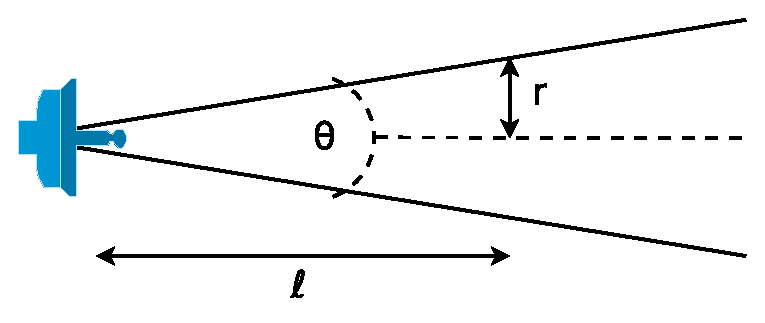
\includegraphics[width=0.5\textwidth]{radiation-cone}
\end{figure}

The datasheet says that the beam-width is less than 3.5°. Let's make a
simplifying assumption that it is exactly that width and further that
the cross-section of the main lobe of radiation is circular. Generally
the radius of the cross-section will be,
\begin{equation}
r = \ell\, \sin(\frac{\theta}{2}) = 10\,\text{m} \times \sin(1.25°) = 0.22\,\text{m}
\end{equation}
The area of this circle is, $\pi r^2 = 0.15 \text{m}^2$.

So now, how much power goes through one square meter when
transmitting at 33 dBm?
\begin{equation}
p = \frac{10^{\frac{\beta}{10}}}{a}  = \frac{10 ^ {33\,\text{dBm}/10}}{0.15\,\text{m}^2} = 
\frac{1995\,\text{mW}}{0.15\,\text{m}^2} = 13.3\,\text{W}/\text{m}^2
\end{equation}
Clearly this is well in excess of the permitted output power.

\subsection{Initial configuration and testing}
\label{december-2013-initial-configuration-and-testing}

\begin{wrapfigure}{r}{0.3\textwidth}
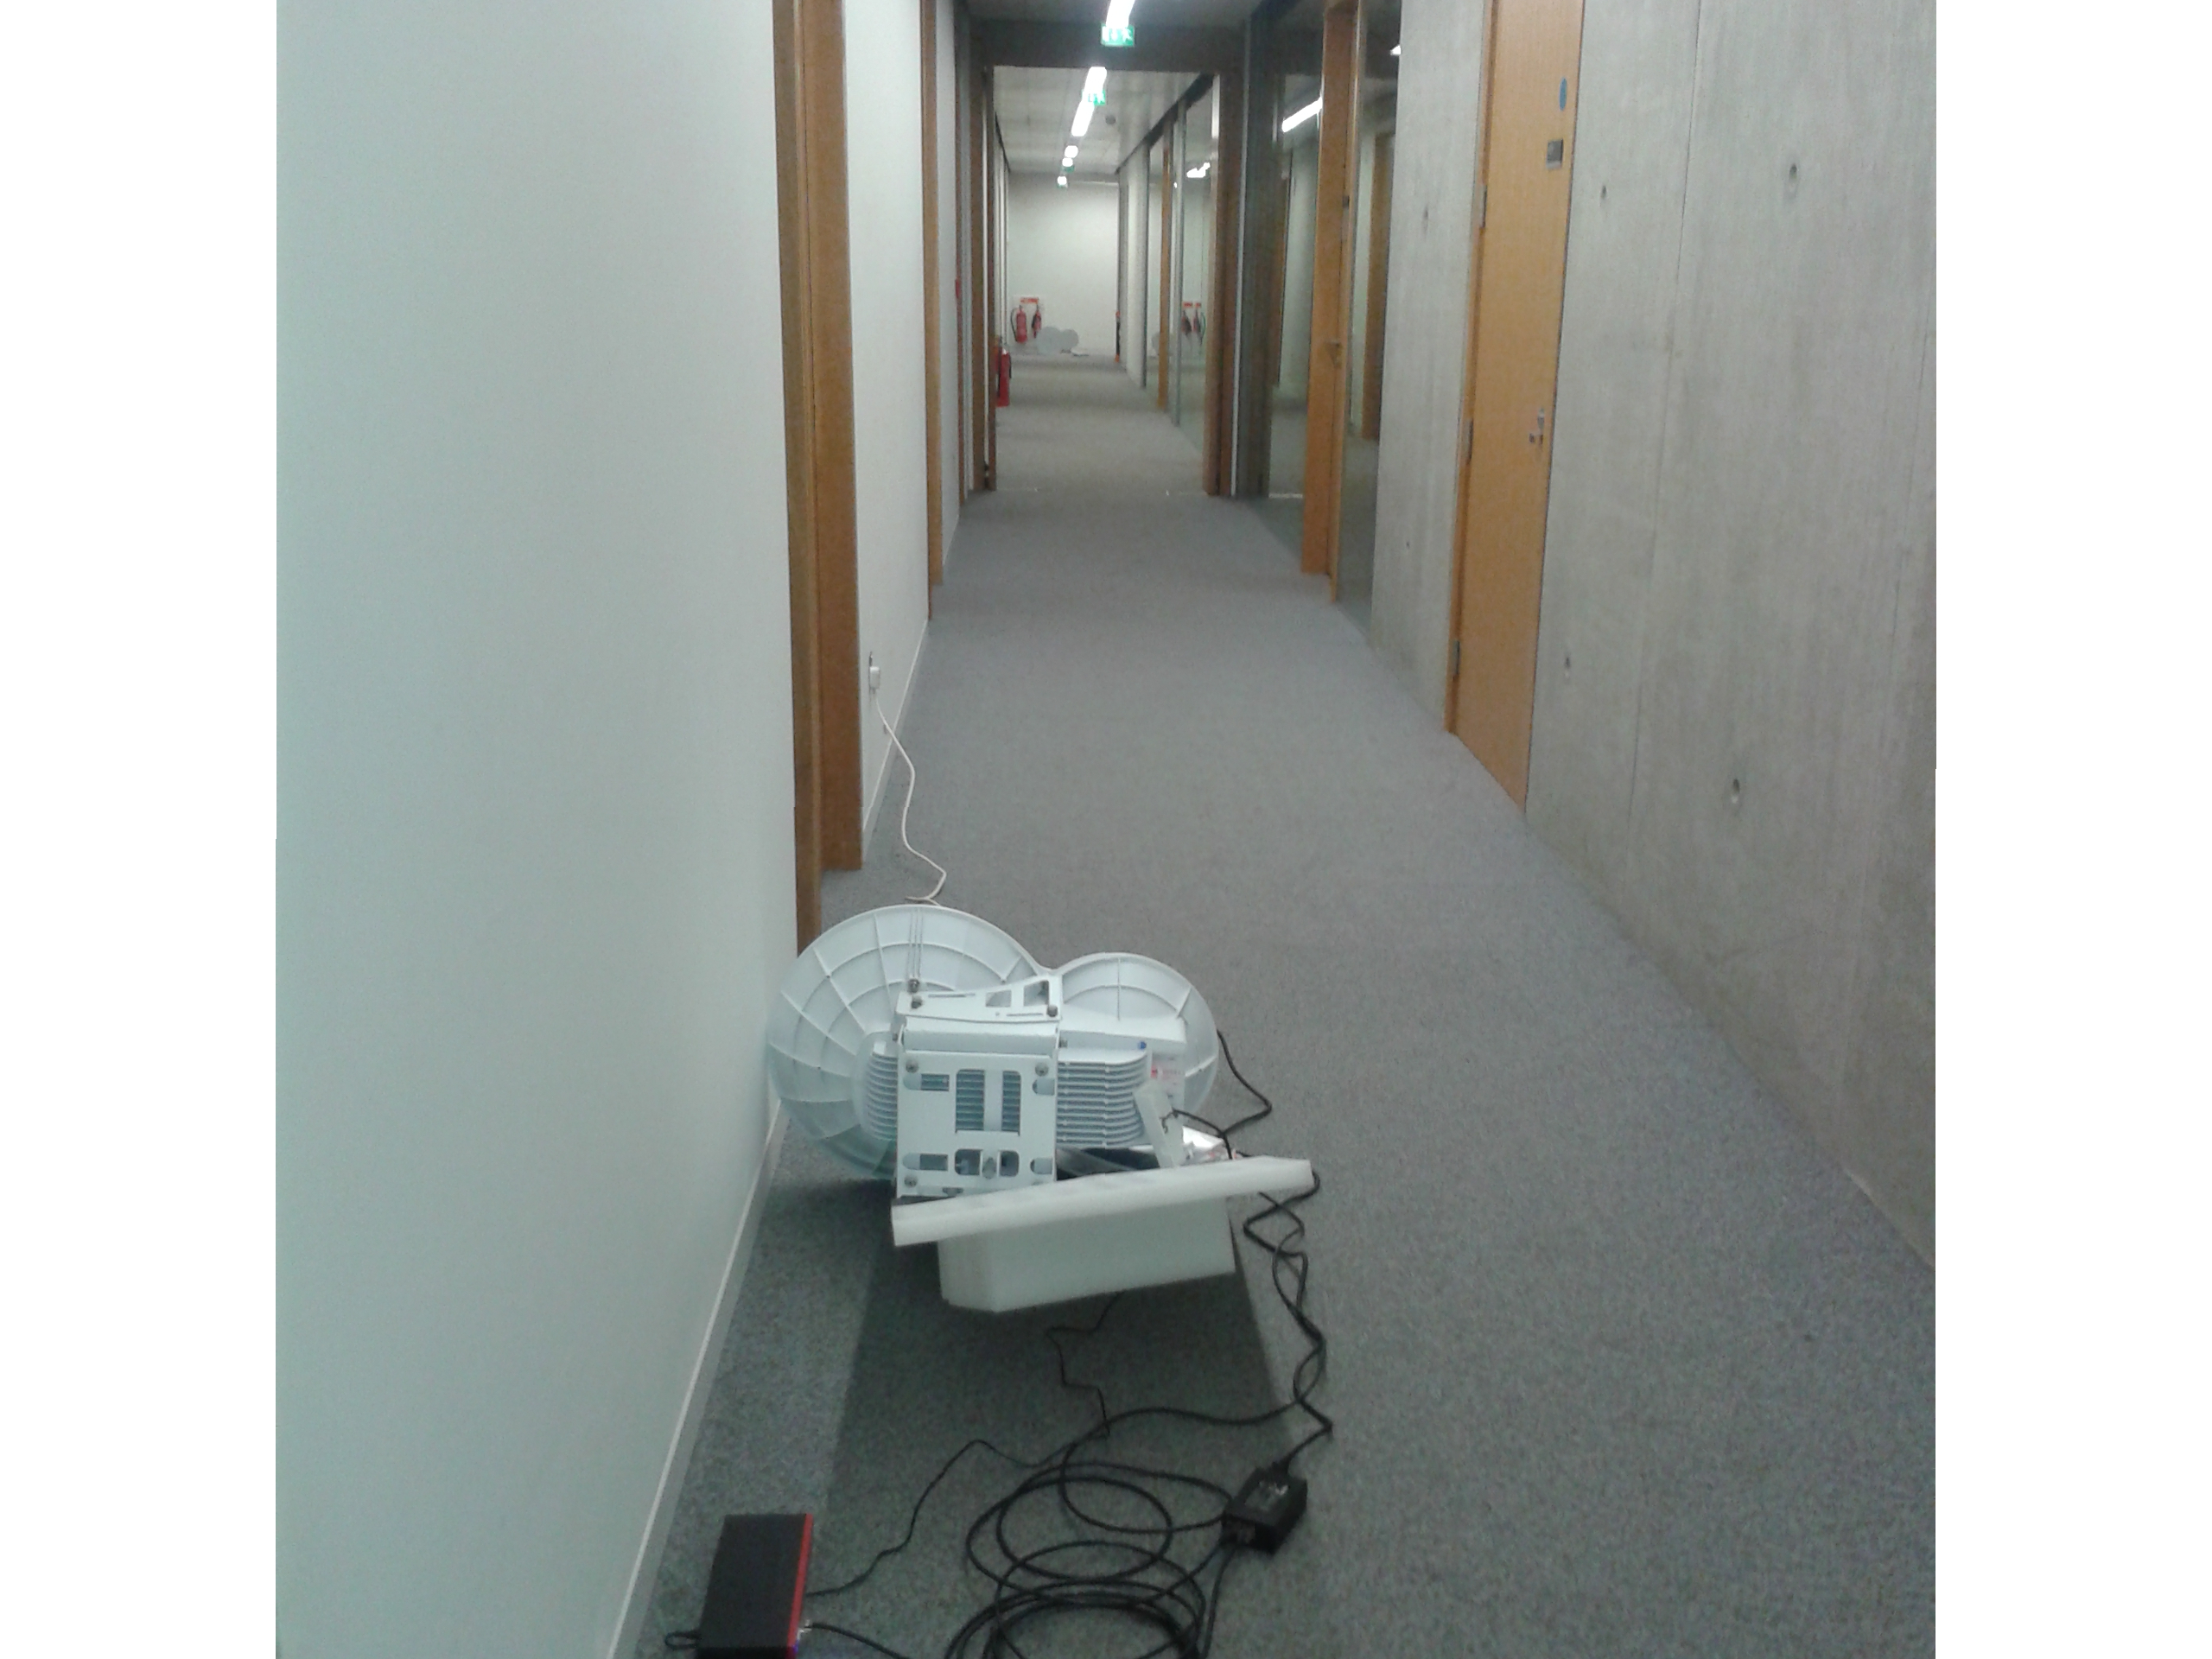
\includegraphics[width=0.3\textwidth]{radio-in-corridor}
\end{wrapfigure}
We ordered and received one pair of radios. Before deploying them
we thought it would be a good idea to check that they were working
and test them in ideal situation -- our office corridor. One thing
we immediately noticed was how critical alignment is. Even over
a distance of 35m, the performance fell of dramatically if the
antennae were slightly out of alignment. It's a very good idea to
configure equipment before deploying it, but to do this we had to turn
off sychronisation which relies on GPS and doesn't work indoors.

\subsection{Strengthening the masts}
\label{december-2013-january-2014-strengthening-the-relays}

Our basic relay construction (see the
\href{http://www.tegola.org.uk/howto/relay-construction.html}{relevant
  howto on the Tegola web site}) uses aluminium pegs to anchor the
diagonal braces to the ground. Both sites were on terrain that
consisted of bedrock covered by peat of varying depth. Although we
have never had a problem with the pegs shifting, peat is a bit
jelly-like, and the structures can wobble through a cm or two. The
alignment of 24GHz is much more critical than for the lower bandwidths
of 2.4 and 5.8GHz, so we replaced the pegs with epoxy bolts into the
bedrock.
\begin{figure}[h]
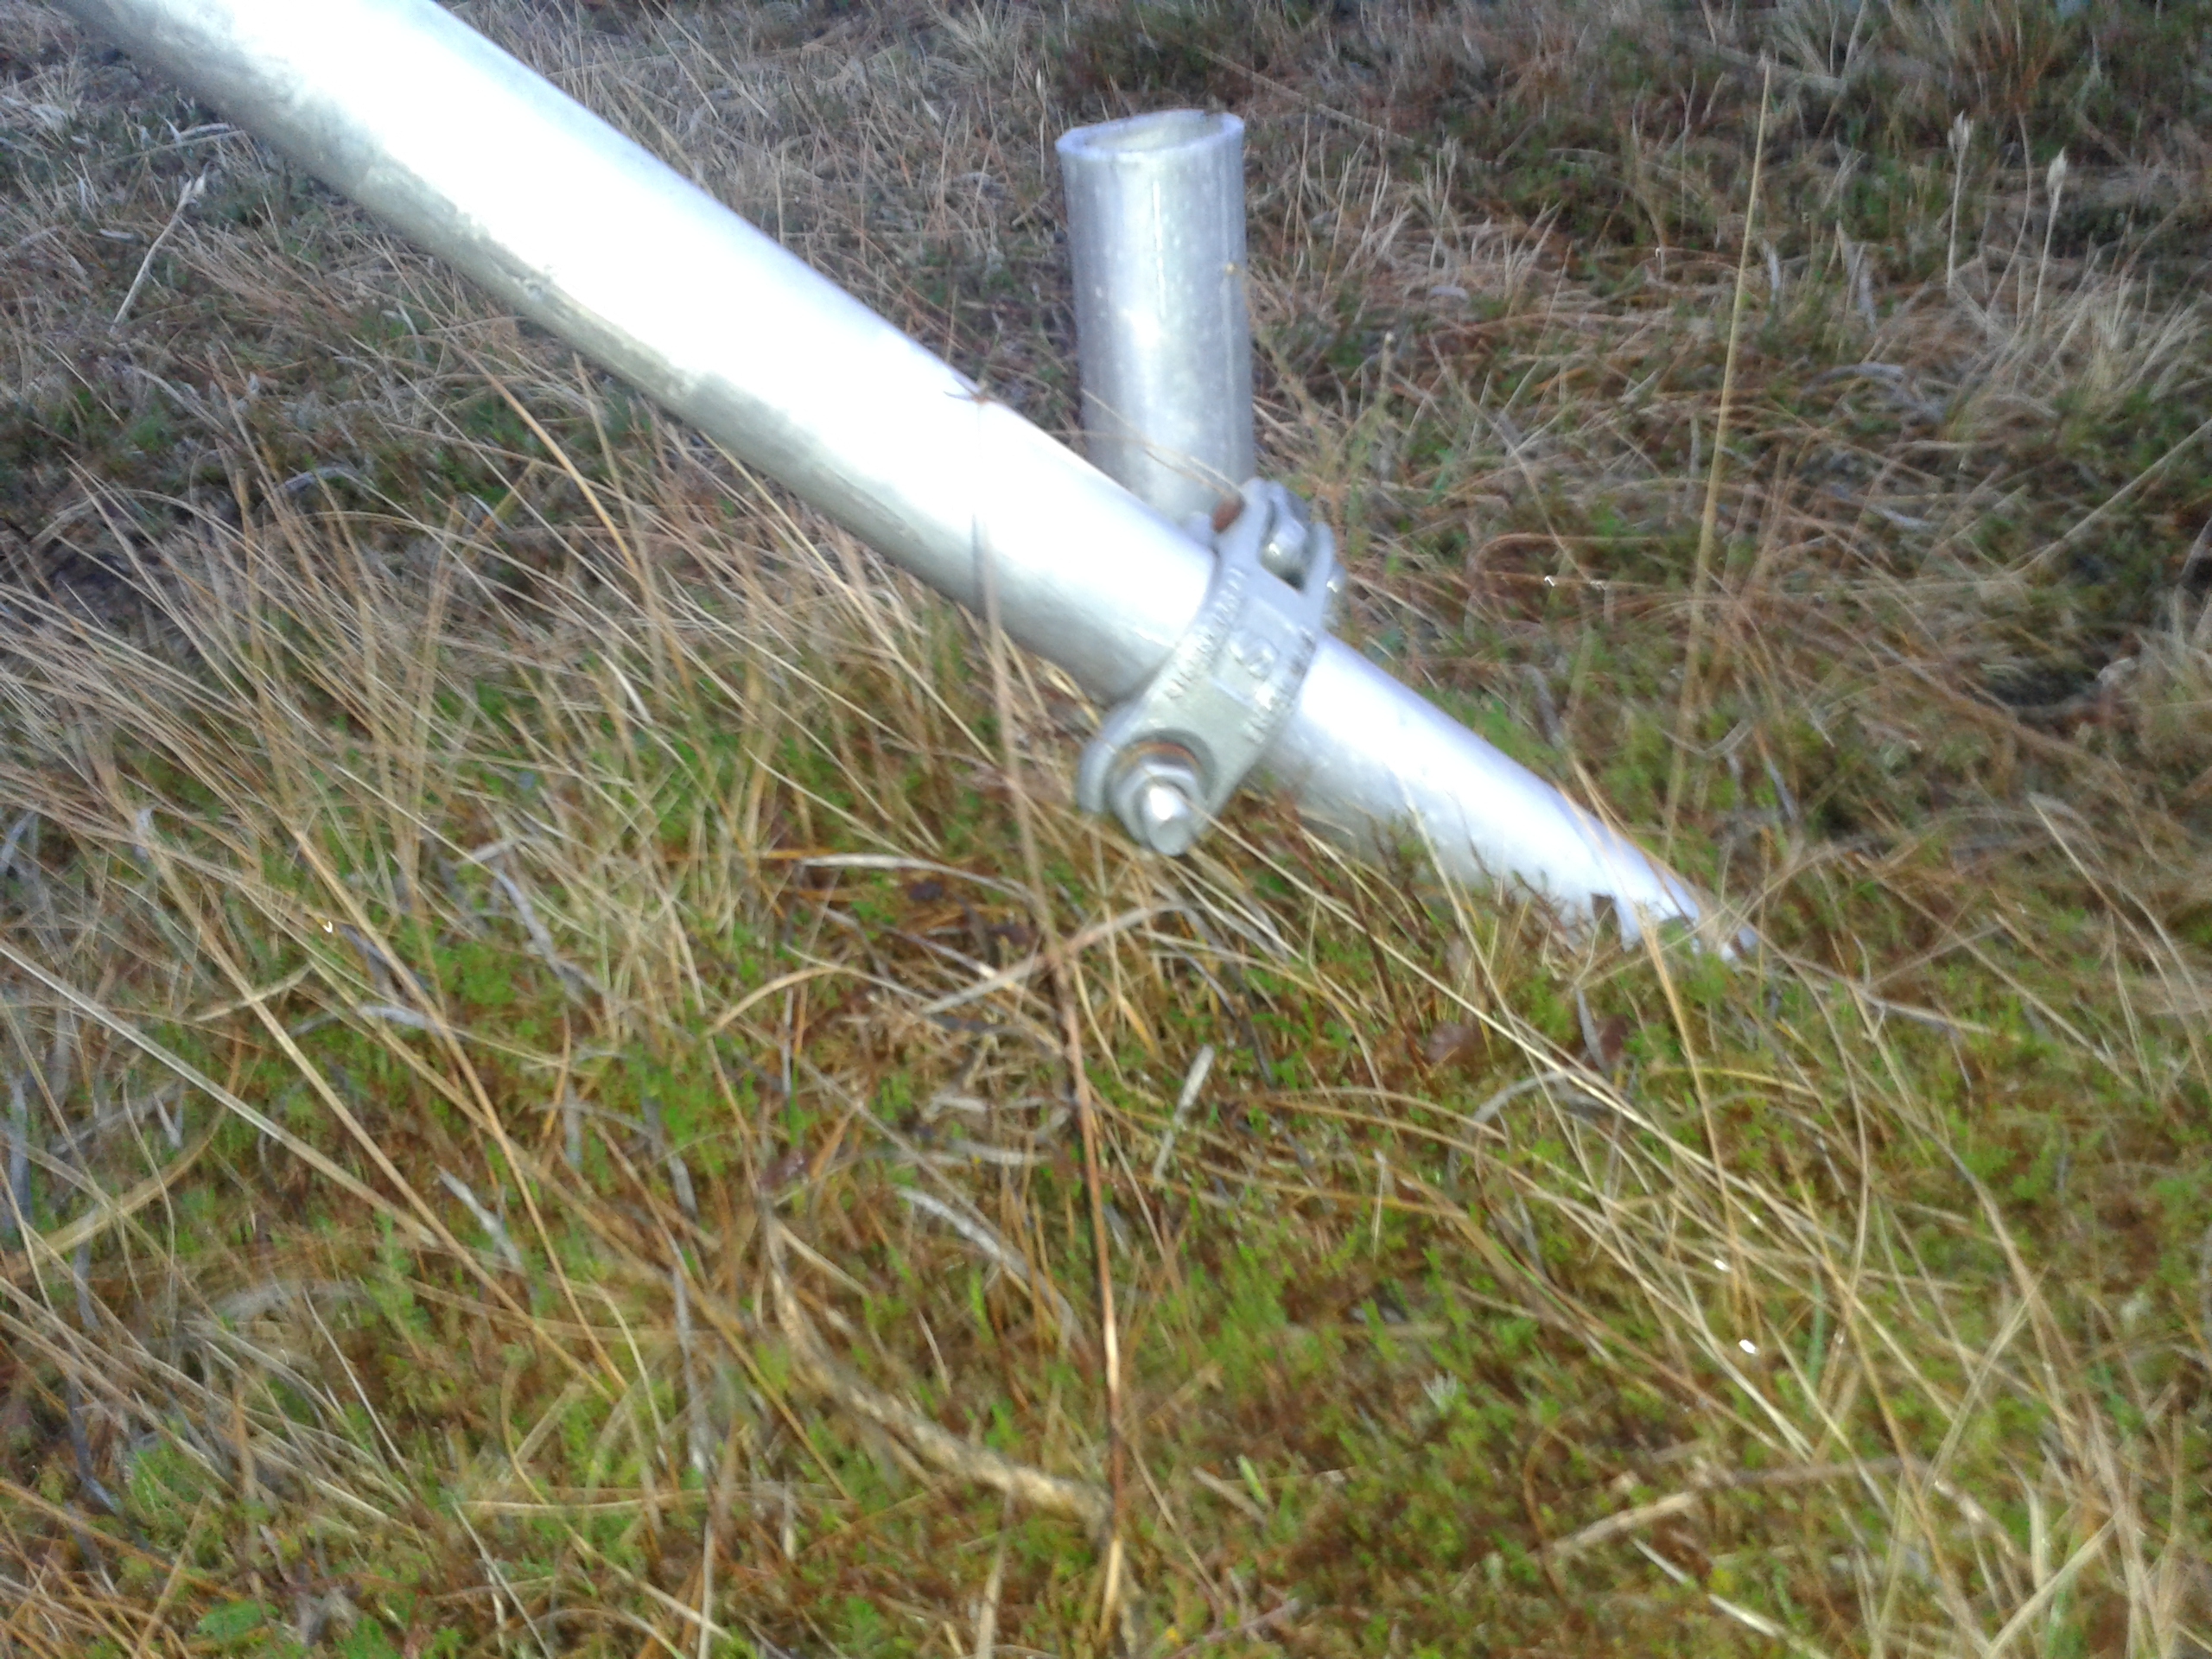
\includegraphics[width=0.4\textwidth]{corran-peg}
\includegraphics[width=0.4\textwidth]{corran-epoxy}
\caption{Pegged anchors (left) and epoxied anchors (right).}
\end{figure}

We also strengthened both relays. For example, at one of our relays we
added an extra horizontal bar.

\begin{figure}[h]
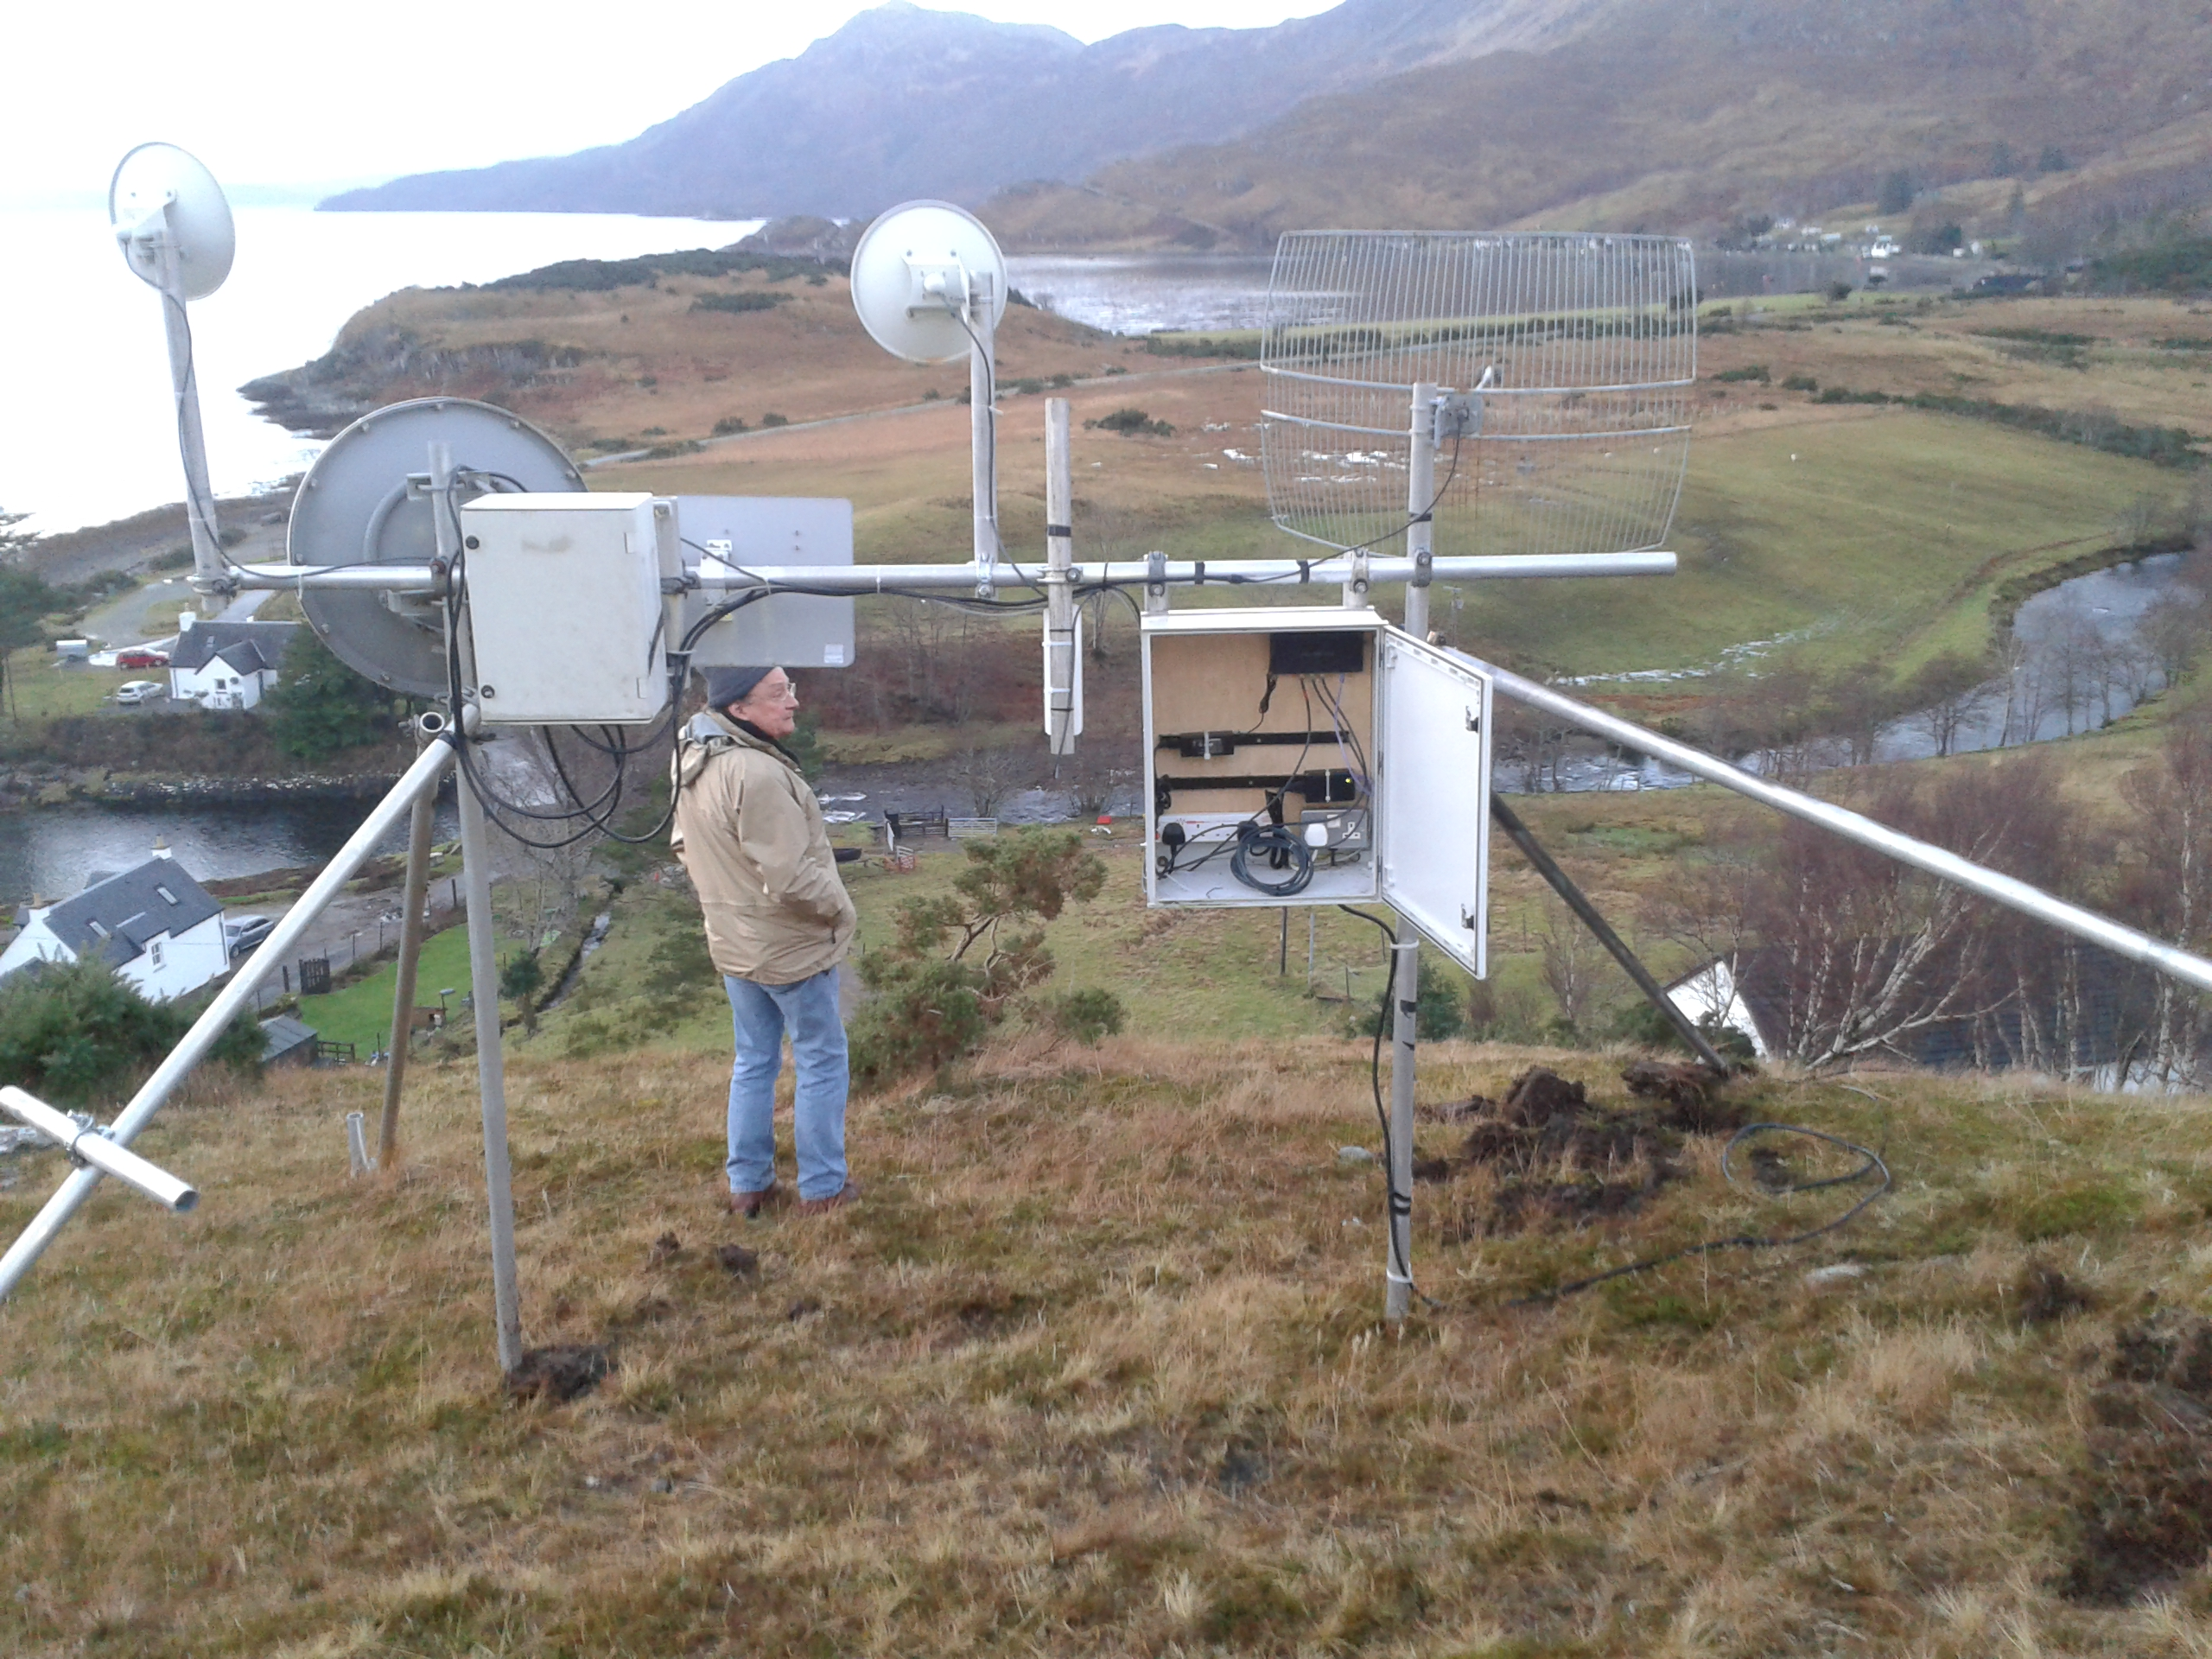
\includegraphics[width=0.4\textwidth]{corran-before-from-behind}
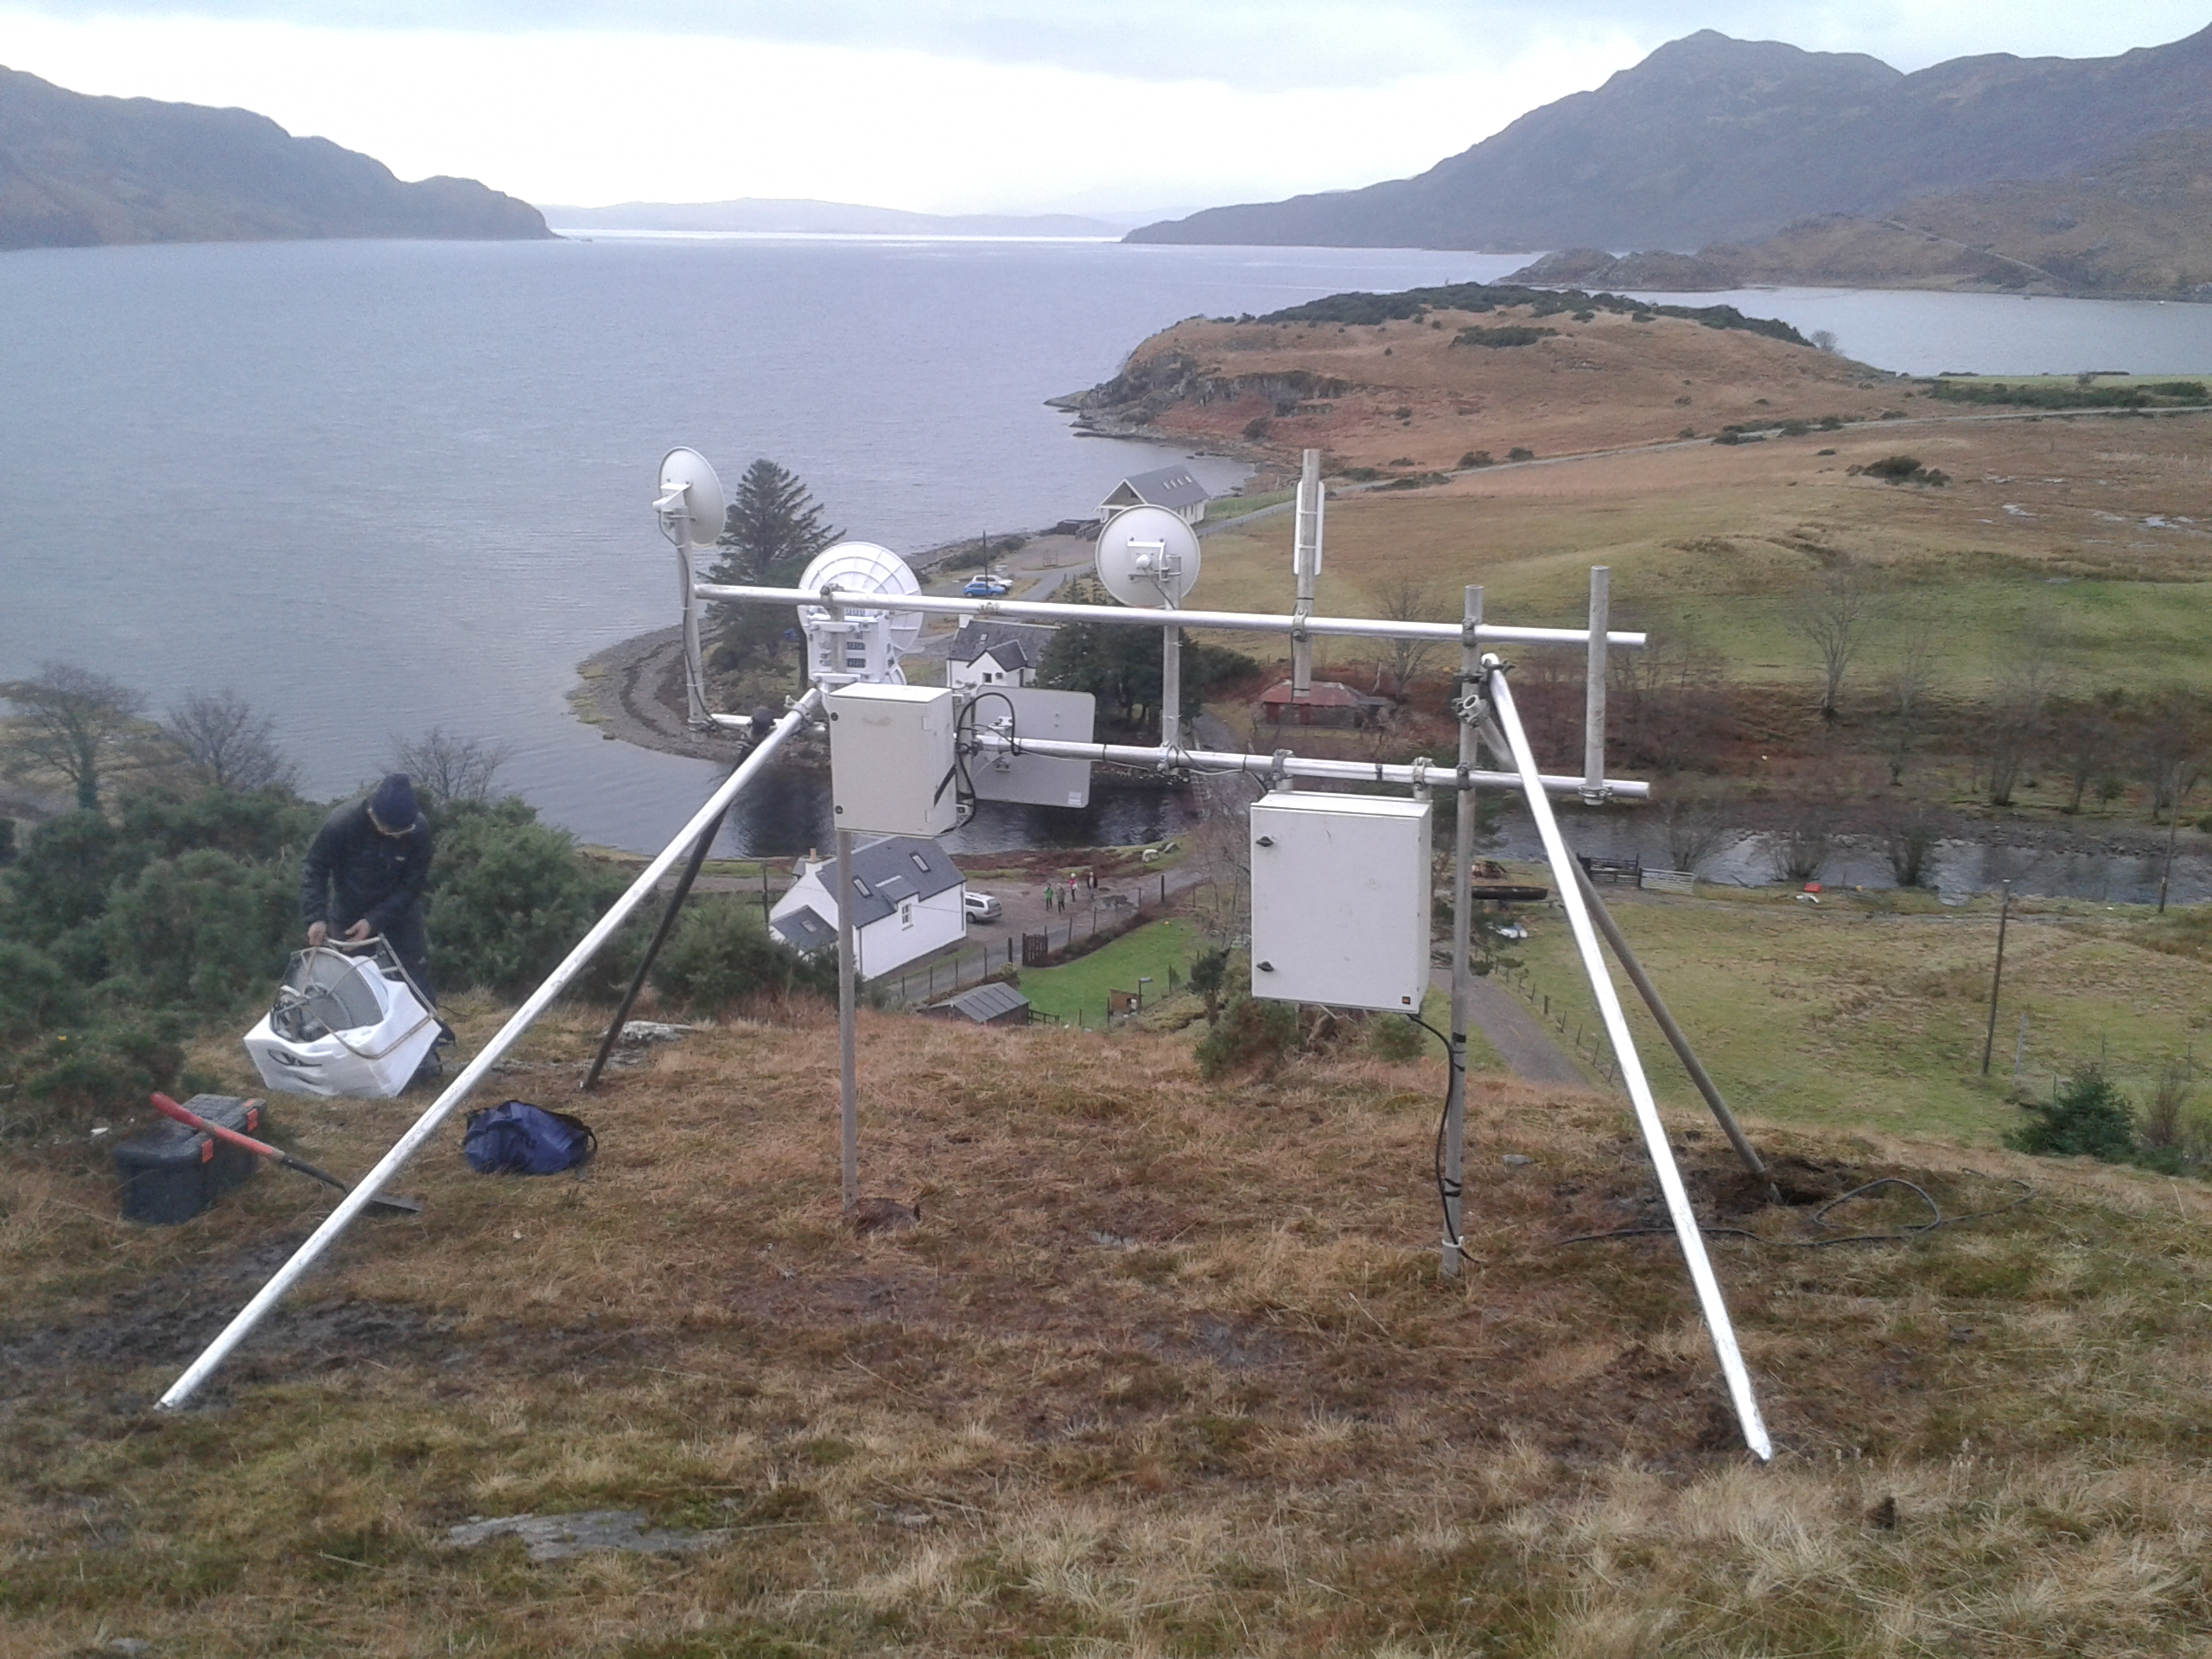
\includegraphics[width=0.4\textwidth]{corran-after-from-behind}
\caption{Corran mast before (left) and after (right)}
\end{figure}

\subsection{Installation and alignment}
\label{january-2014.-installation-and-alignment}

The radios are reasonably light (under 10kg) but awkward to carry up
hills. We used an old backpack frame that 30 years ago had been used
for carrying batteries up to community TV relays. The radios come with
a mounting frame that is first attached to the structure. The radio is
then ``slotted'' into the mounting frame. This arrangement makes it
quite easy to install the whole assembly when working from a ladder.

The antenna can be aligned through elevation and azimuth
adjustment screws. Unfortunately there is a great deal of backlash in
these screws, and they are almost useless if you are working in high
winds. If the clamping bolts are loose, the antenna is blown around
through the considerable travel allowed by the adjustment screws. The
signal strength read-out is at the bottom of the antenna, and if
the alignment is being done from a ladder, you almost certainly
need someone below (with a hard hat) to squint up and call out
the figures.

The installation instructions recommend an alternating process in which
one end of the link is adjusted then the other, and so
on. Unfortunately we were unable to complete this process before
the weather closed in and our workforce departed. However, the
alignment is good enough that we can start taking some measurements.
The initial indications are that the link will work reasonably well
over a distance of 6.5km.

\subsection{Performance}\label{performance}


\section{Free-space Optics}
\label{sec:fso}

The purpose of the trials with the free-space optical (FSO) links was to
ascertain the extent to which fog, a common feature of the Scottish
environment especially in coastal areas, would affect their
use. Obviously fog would attenuates the signal to some extent since
the units operate in the near-infrared spectrum. We can quantify this
effect theoretically as we do in \S\ref{sec:absorption} and
\S\ref{sec:scattering},
but we were primarily interested in finding out if their operational
window was, on average, large enough to justify the considerable
expense.
\begin{figure}
  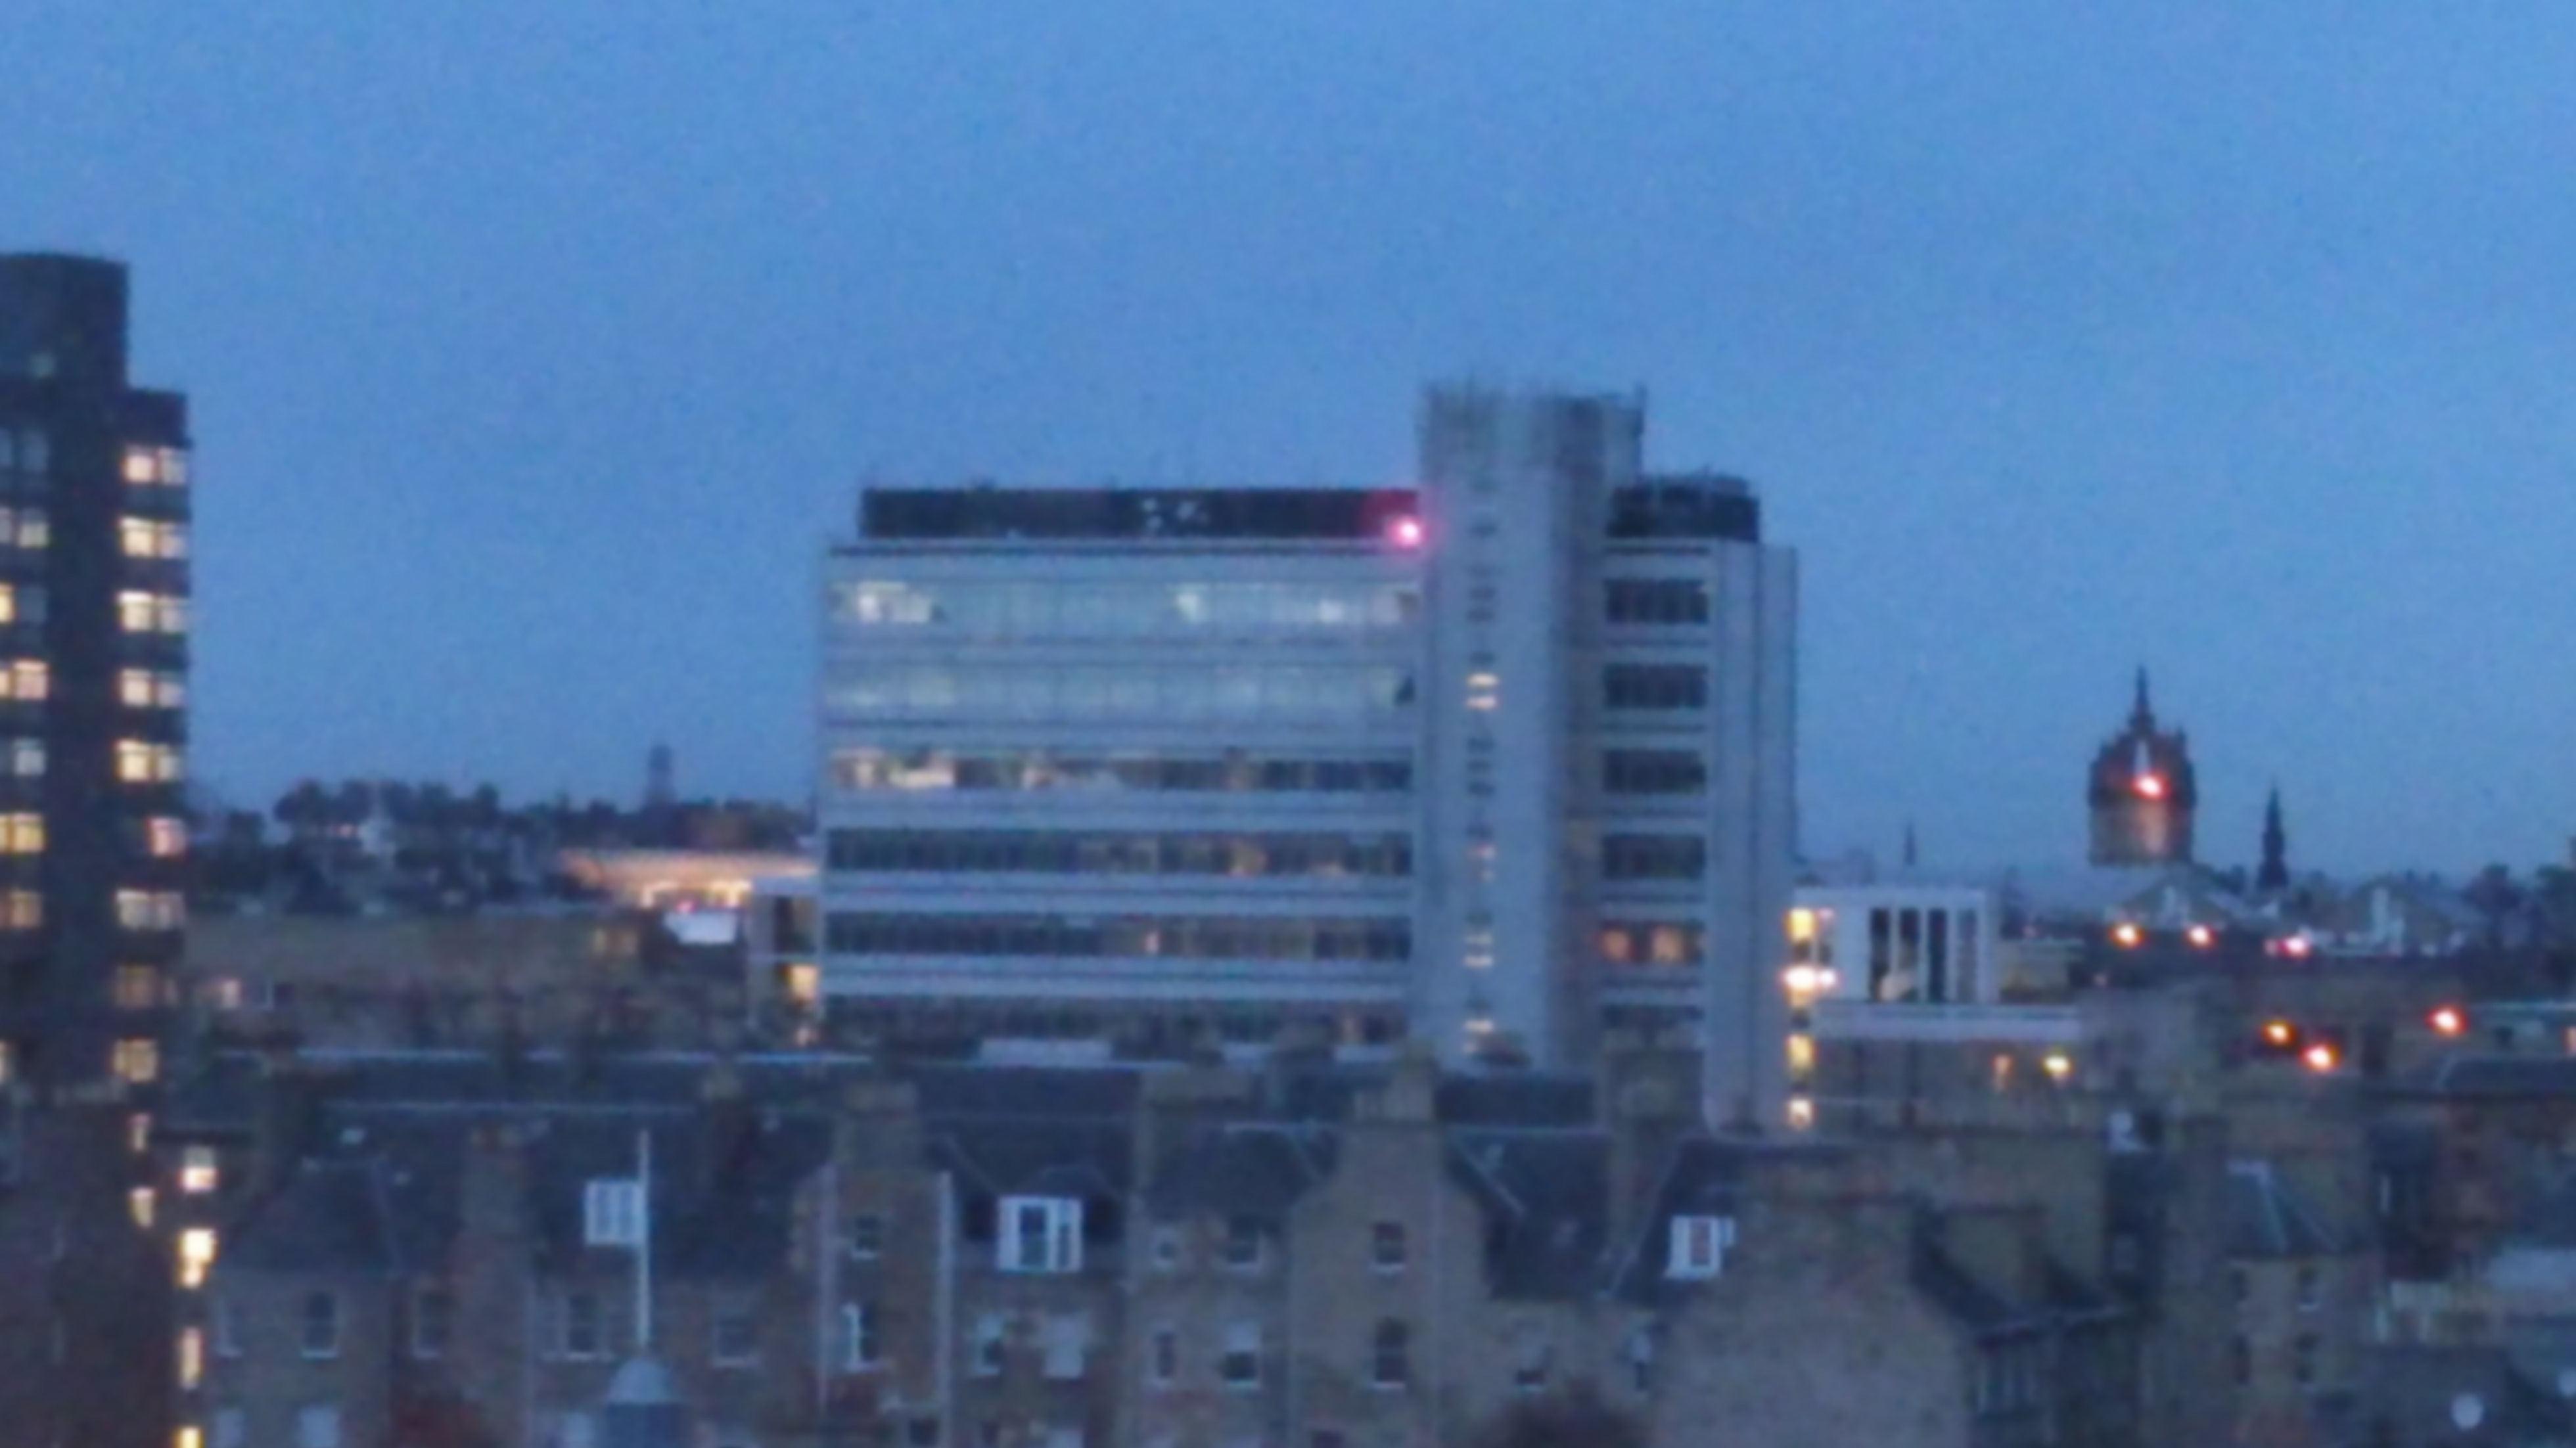
\includegraphics[width=\textwidth]{at-laser.jpg}
\end{figure}

The Scottish Government had a preferred vendor, CableFree, for the
equipment though we were formally free to select another. Our budget
was only about \pounds 10,000 for the equipment. The FSO vendors that
are well-regarded in industry such as F-Sona and Canon do not produce
anything in this price range. Small wonder as their primary market is
the military -- optical links are much harder to eavesdrop upon
compared to radio links. Two vendors were within our price range:
Geodesy of Hungary and Cablefree.

We selected the suggested vendor partly because they were a local
(i.e. UK-based) company on the theory that they might be more
responsive and accessible. We were also given to believe -- with no
evidence -- that their Hungarian competitor used inferior, older
technology. It is difficult to tell the extent to which this was
true without comparing the equipment from both manufacturers side by
side. We were subjected to the hard-sell and given very little
concrete information without signing non-disclosure agreements that
would prevent our conducting any useful research. As it was, not
executing the NDAs prevented us from properly instrumenting the
equipment and measuring its behaviour at any but very coarse
granularity.


The whole episode was without a doubt the most unpleasant interaction
with an equipment vendor in our considerable experience.

\subsection{Link Design}
\label{sec:link-design}

CableFree produced a link design as shown in
Figure~\ref{fig:cablefree-link}. In principle it is plausible,
consisting of a laser link, and a back-up radio link between Appleton
Tower and the Tech Cube, a distance of about 500m. At either end two
switches would use the spanning-tree protocol (STP) configured with the
radio link having a higher cost than the laser link. The principle
being that traffic would flow over the lasers unless they were
unavailable in which case the backup link would be used.
\def\cfdesign{%
    \node[draw,rotate=90] (atnetgear) at (0,0) {Netgear Switch};
    \node[draw] (atlaser) at (2,1) {Laser};
    \node[draw] (atradio) at (2,-1) {Radio};
    \node[draw] (tclaser) at (6,1) {Laser};
    \node[draw] (tcradio) at (6,-1) {Radio};
    \node[draw,rotate=-90] (tcnetgear) at (8,0) {Netgear Switch};
    \draw[thick,blue] (-1,0) edge (atnetgear.north);
    \draw[thick,blue] (9,0) edge (tcnetgear.north);
    \draw[thick,orange] (atnetgear.south) edge (atlaser.west);
    \draw[thick,orange] (tcnetgear.south) edge (tclaser.east);
    \draw[thick,blue] (atnetgear.south) edge (atradio.west);
    \draw[thick,blue] (tcnetgear.south) edge (tcradio.east);
    \draw[thick,red,dotted] (atlaser.east) edge (tclaser.west);
    \draw[thick,black,dotted] (atradio.east) edge (tcradio.west);
    \node at(4,0) {$\approx 500\text{m}$};
    \node at(4,1.5) {$\text{cost} = 1000$};
    \node at(4,-1.5) {$\text{cost} = 100000$};
}
\begin{figure}[h]
  \centering
  
\begin{tikzpicture}
    \node at (1,2) {\textbf{Appleton Tower}};
    \node at (7,2) {\textbf{Tech Cube}};
    \cfdesign
  \end{tikzpicture}
  \caption{CableFree Link Design}
  \label{fig:cablefree-link}
\end{figure}

There were, however, several problems with this design. The less
serious was that this design was hardly appropriate for the local
environment. We already had a significant amount of radio equipment at
both sites -- including a radio link between them -- so an extra radio
link was superfluous. The radios specified by the vendor were low-end
Mikrotik radios with panel antennae in a waterproof enclosure. This is
not to cast aspersions on Mikrotik equipment, indeed we make much use
of it and it is generally quite good for the price. However Cablefree
wished to sell this re-branded equipment at a significant markup.

\begin{wrapfigure}{r}{0.3\textwidth}
  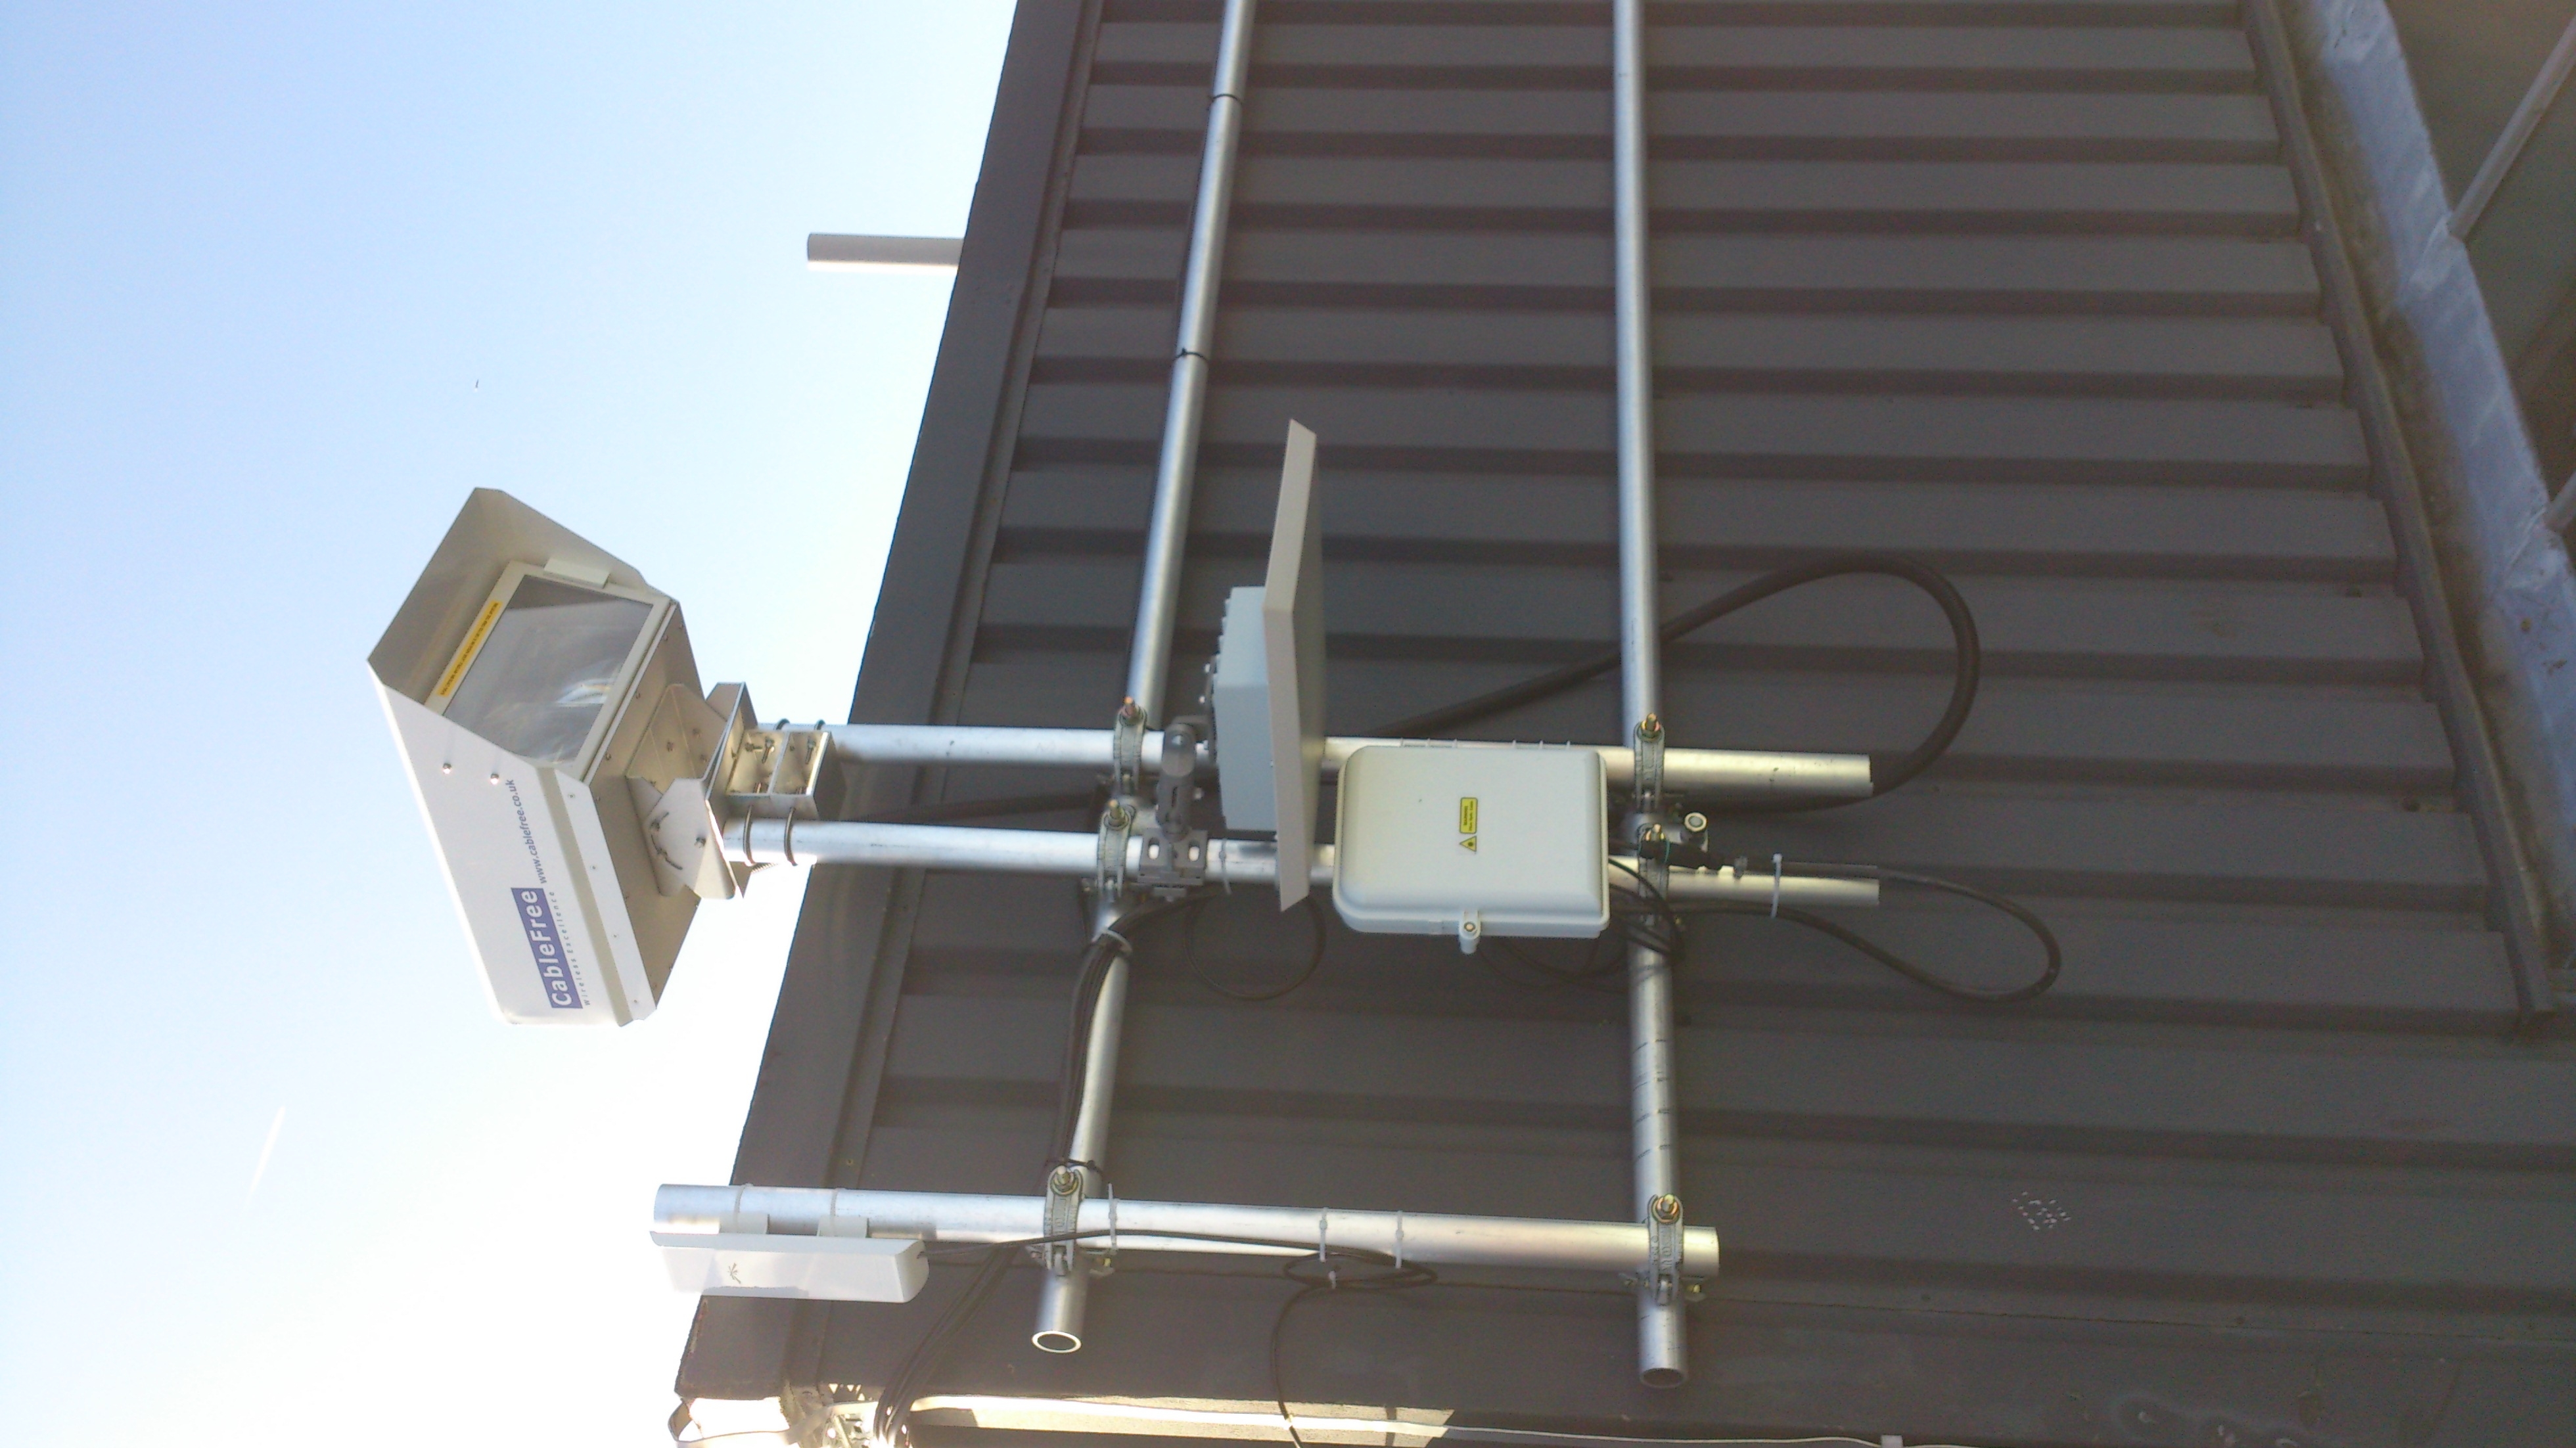
\includegraphics[angle=-90,width=0.3\textwidth]{also-faulty}
\end{wrapfigure}
Most amusingly, the mounting brackets supplied with the re-branded
Mikrotik radios were somewhat flimsy. It can get very windy at the top
of tall buildings in Edinburgh. Wind speeds can reach several times
more than at ground level. The installation is shown at right with the
mounting bracket having worked loose in high winds leaving the radio
pointing downwards.

We also had high end HP ProCurve J9050A switches at either end (loaned
by the School of Informatics), far more capable network elements than
the consumer-grade Netgear switches (see
Figure~\ref{fig:carrier-grade}) specified by the vendor. The
deficiencies of the Netgear switch are that it is not manageable via
telnet or ssh, which makes it very difficult to recover from outages
or erroneous configurations in a network of any size or complexity,
and more seriously, the cheap power adapter of the kind that are prone
to failure or simply disconnection due to the use of barrel
connectors. The power injector for the re-branded Mikrotik radio also
suffers from this deficiency (the white apparatus connected into the
switch in the photograph).

Unfortunately CableFree wished to sell a ``complete solution'' for us
to evaluate rather than an ``appropriate solution'' for our
circumstances and we succumbed to their hard-sell, ``complete'' with
sub-standard parts. We ultimately ended up operating the link by
connecting the vendor-supplied netgear switches to our HP switching
core and removing the vendor-supplied radio equipment entirely.
\begin{figure}
  \begin{center}
    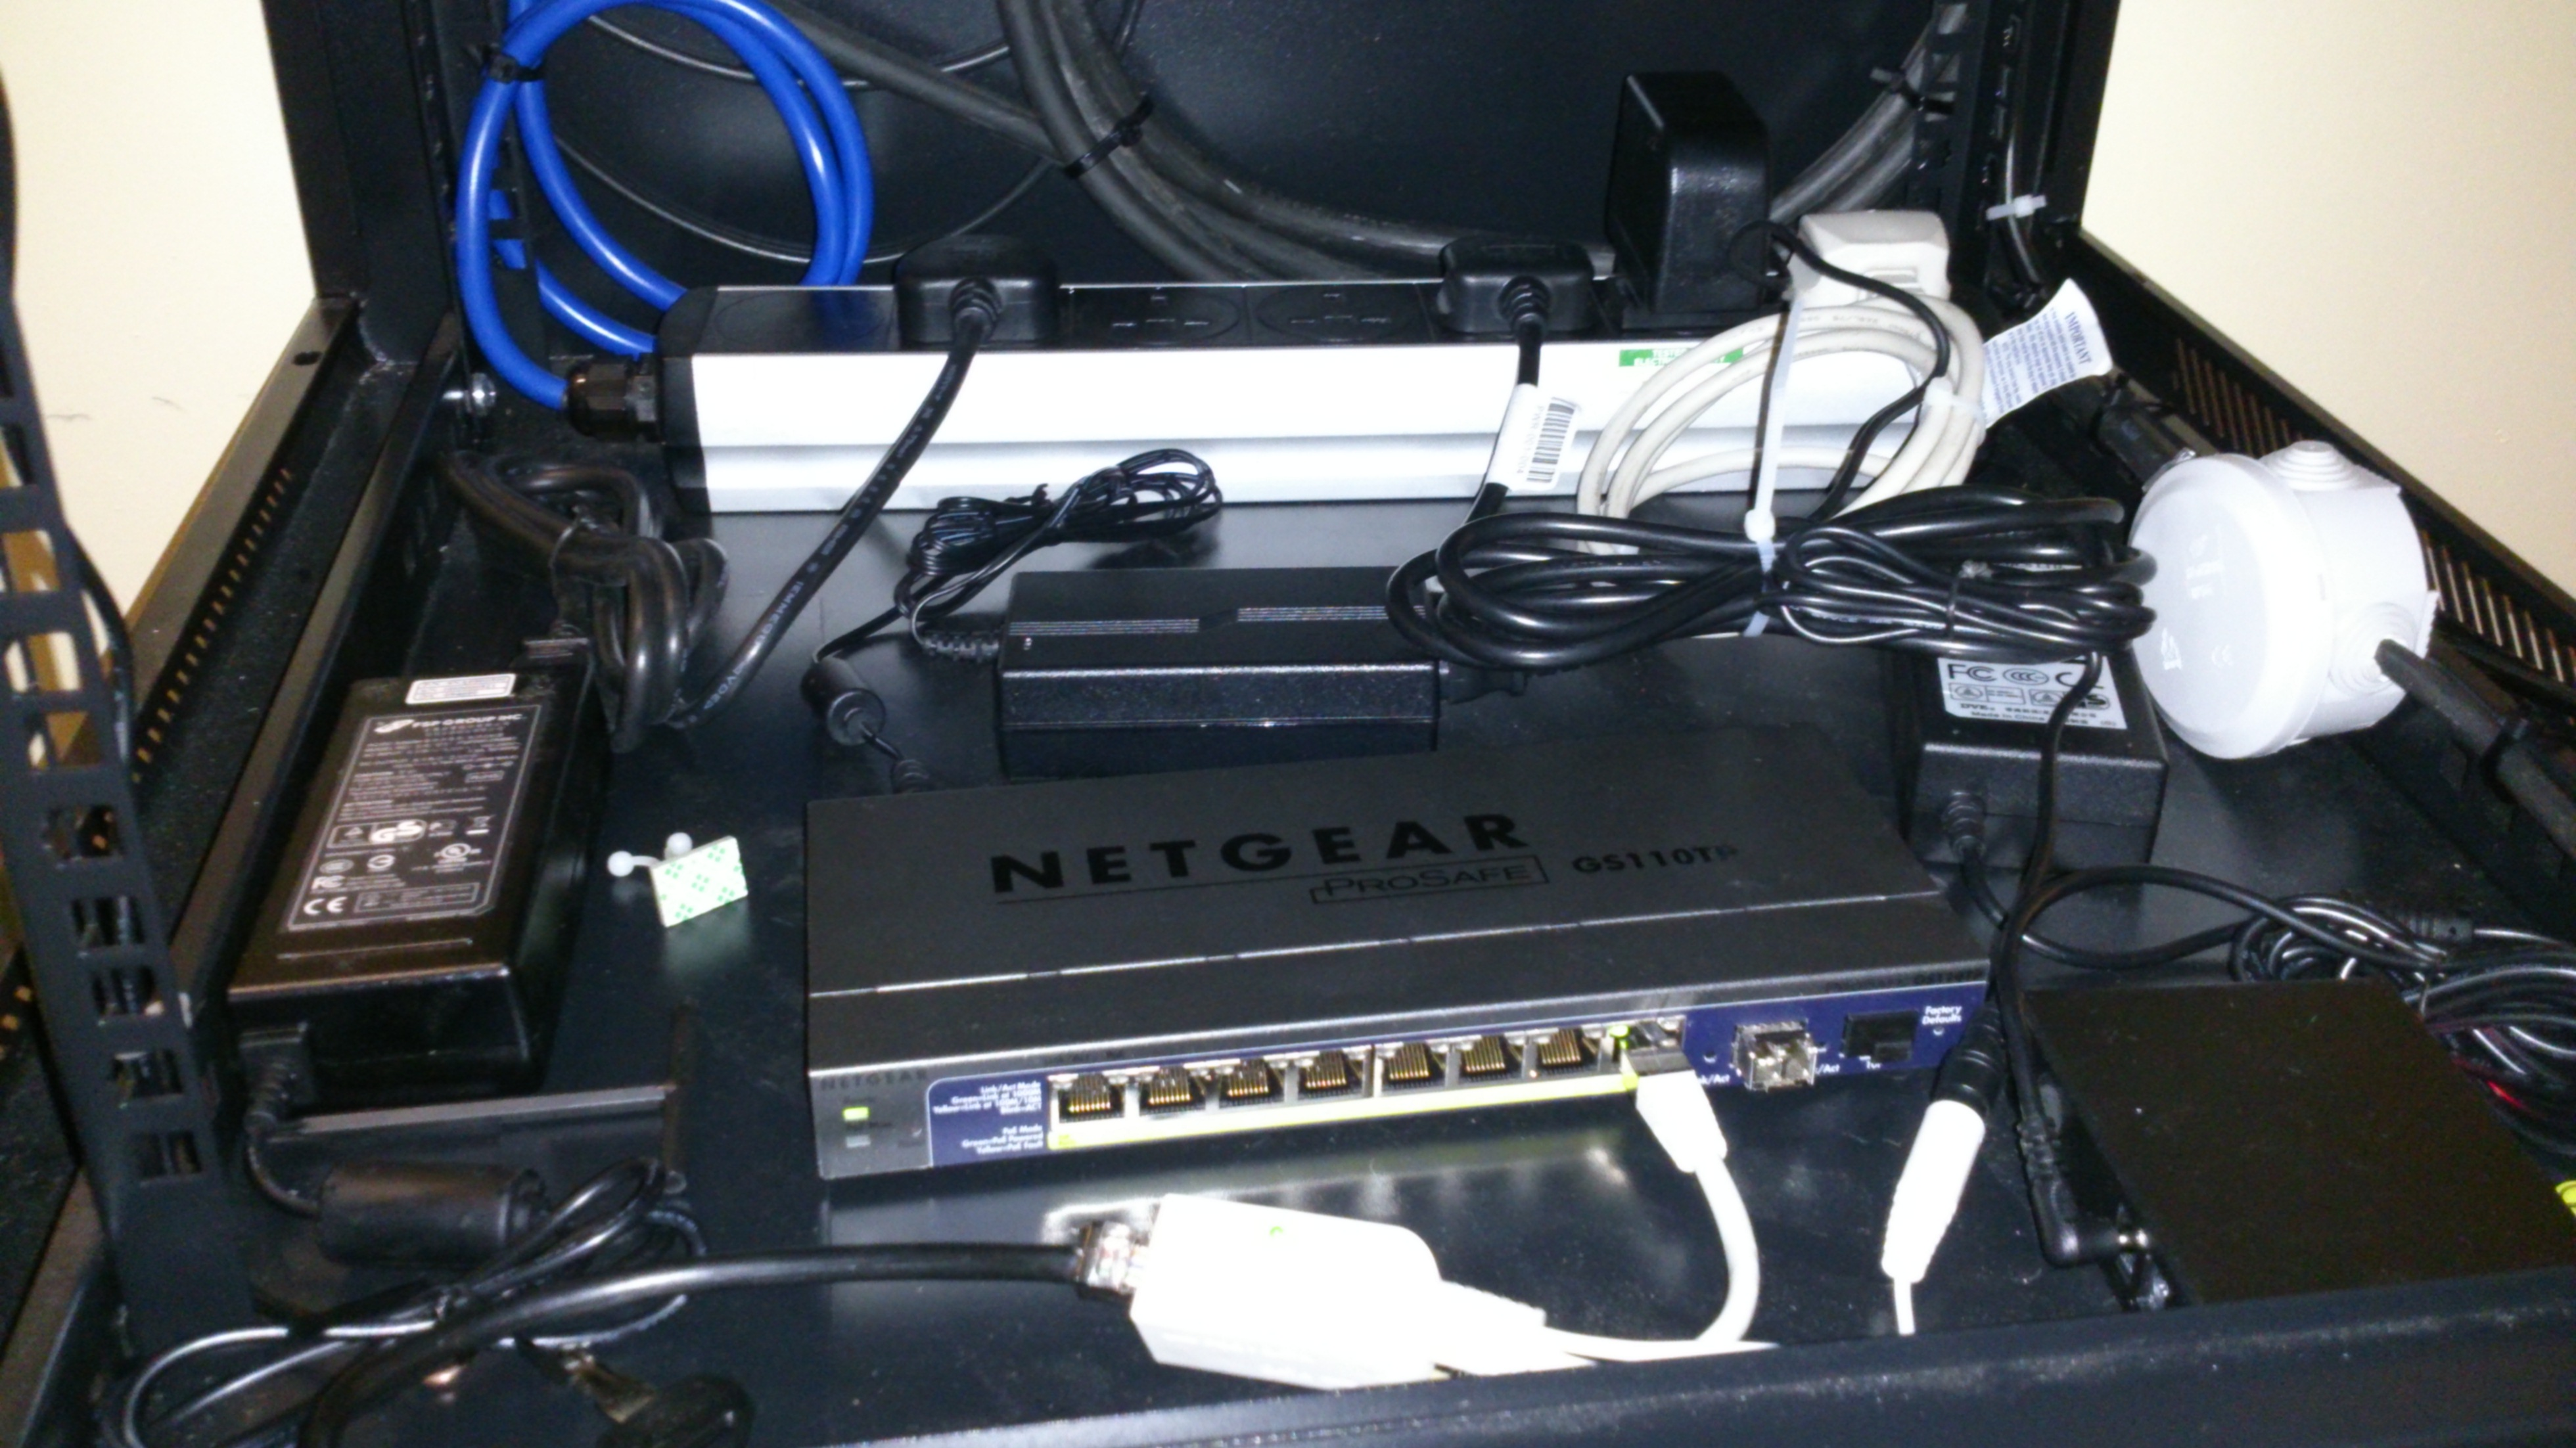
\includegraphics[width=0.5\textwidth]{carrier-grade}
  \end{center}
  \caption{A ``carrier-grade'' ethernet switch.}
  \label{fig:carrier-grade}
\end{figure}

The more serious deficiency with this design is the use of the
spanning-tree protocol. We will have more to say about the detail of
this below, but in brief, the mechanism is unstable in marginal
conditions. If the weather is clear or if the weather is very foggy,
the link operates as designed. However in the region between clear and
very foggy, the path is liable to rapidly change between the (possibly
unuseable) optical link and the radio link. Evidence for this is
anectodal due to the impossibility of properly instrumenting the
optical equipment, of which also more below.
\clearpage

\subsection{Absorption of light by water}
\label{sec:absorption}

Unlike electromagnetic waves at radio frequencies which are not
significantly attenuated by atmospheric gasses, in the visible and
near-infrared part of the spectrum this effect plays a major role. We
all know from our experience that this is the case, for example this
effect explains why objects under water take on a blue-green tinge --
because the red part of the light reflected from them is attenuated
more by water than blue or green light. In fact we have data for this
which is shown plotted in Figure~\ref{fig:absorption-liquid} which
ranges over wavelengths from the ultraviolet (circa 380nm) to the
near-infrared (circa 800nm).
\begin{figure}[h]
  \centering
  \begin{tikzpicture}
    \begin{axis}[
      xlabel={Wavelength $\lambda$ in $\mu$m},
      ylabel={Absorption coefficient $\alpha$ in $\text{m}^{-1}$},
      xmin=0.380, xmax=0.800,
      ymin=0, ymax=3
      ]
      \node[coordinate, pin=-55:{$\alpha \approx 2.65$}]
          at (axis cs:0.380,2.65) {};
      \node[coordinate, pin=165:{$\lambda = 780\,\mu\text{m}$}]
          at (axis cs:0.780,0) {};
      \addplot[blue,thick] table {water.dat};
      \draw[red] (axis cs:0,2.65)
                    to (axis cs:0.78,2.65)
                    to (axis cs:0.78,0);
    \end{axis}
  \end{tikzpicture}
  \caption{Absorption of light by frequency through liquid water
    (\cite{jonasz_absorption_2007})}
  \label{fig:absorption-liquid}
\end{figure}

A line is marked on the diagram that shows the particular wavelength
of interest for the free-space optical equipment, 780nm. This
corresponds to an absorption coefficient of around 2.65/m$^{-1}$ which
means that through liquid water, light at this wavelength decreases in
intensity by 2.65 times for every meter of water that it travels
through.

We are not, however, intending to operate this equipment under
water. Instead we are interested in water vapour in the form of clouds
or fog, so we need to figure out how much water vapour is contained
in a given amount of air when a cloud is present. We will take cloud
formation to mean (greater than) 100\% relative humidity. This means
that the vapour pressure of water in the air is greater than the
equilibrium vapour pressure at which it evaporates and condenses at
equal rates. In fact it condenses faster than it evaporates and so the
air becomes full of condensed water droplets, or in other words a
cloud forms. The formula for this pressure commonly used in the
literature is given by~\cite{buck_new_1981} as,
\begin{equation}
  \label{eq:buck}
  e_w = (1.0007 + 3.46\times 10^{-6}P)\times 6.1121e^{\frac{17.502T}{240.97+T}}
\end{equation}
with the pressure $P$ given in hPa and the temperature in
$^\circ$C. This relation is plotted in figure{fig:water-pressure} for
a pressure of one atmosphere.
\begin{figure}[h]
  \centering
  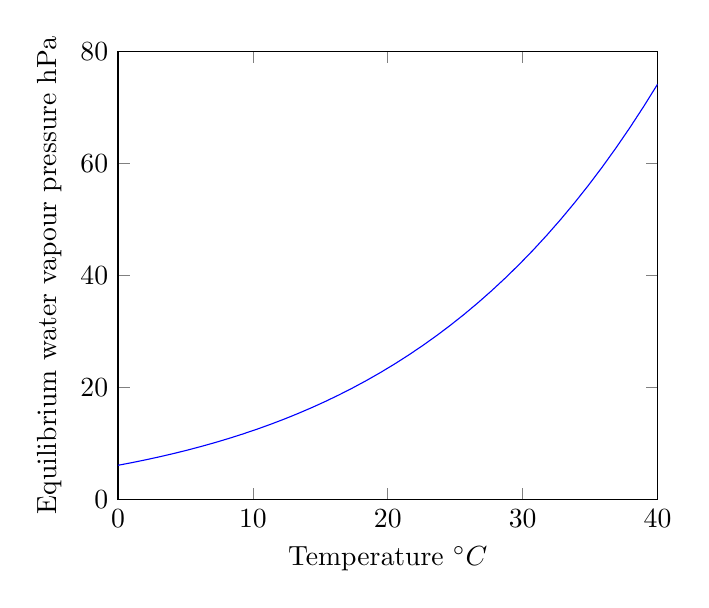
\begin{tikzpicture}
    \begin{axis}[
      ymin=0, ymax=80,
      xmin=0, xmax=40,
      xlabel={Temperature $^{\circ}\text{C}$},
      ylabel={Equilibrium water vapour pressure hPa}
      ]
      \addplot[blue,domain=0:40, samples=40]
              { (1.0007 +
                3.46e-6*1013.25)*6.1121*exp(17.502*x/(240.97+x)) };
    \end{axis}
  \end{tikzpicture}
  \caption{Water vapour density as a function of pressure}
  \label{fig:water-pressure}
\end{figure}

Since this is the minimum water vapour pressure required to form a
cloud, we may take this as a lower bound on the amount of water in the
air. At 10$^\circ$C, Buck's relation gives an equilibrium pressure of
1.23 kPa. Recalling our ideal gas law from high school,
\begin{equation}
  \label{eq:ideal-gas}
  PV = nRT
\end{equation}
we can work out that,
\begin{equation*}
  n = \frac{PV}{RT} 
    = \frac{1.23\times 10^3 \times 1}
           {8.314 \times 283}
    = 0.528\, \text{mol}
\end{equation*}
we can look up the molar mass of water, which is
18.02$\text{g}/\text{mol}$, and so arrive at a density of water in the
cloud as it is forming of 9.01$\text{g}/\text{m}^3$.

So what? Well, we know that, roughly, liquid water has a density of
1$\text{g}/\text{cm}^3$ and in terms of cubic meters this is
$10^6\text{g}/\text{m}^3$. So this tells us that we should scale the
absorption factor for water by $9.01\times 10^{-6}$ at the point of
cloud formation, which gives an adjusted absorption factor of
$2.39\times 10^{-5}$. Over the course of our 500m path, this means
that loss due to absorption (heating of the cloud) is only about
1\%.

In practice, this value is an overestimate, owing primarily to the
fact that water vapour does not behave as an ideal gas near the phase
transition from vapour to water (condensation). Experimental
measurements (\cite{whiteman_cloud_1999}) and more sophisticated
models (\cite{tampieri_size_1976,hess_optical_1998}) give values a
couple of orders of magnitude lower for the density of water in
fog. We therefore conclude that absorption is not a significant factor
in attenuation of the signal from the lasers by fog.

\subsection{Scattering of light by water}
\label{sec:scattering}
Another possible effect on the light of the lasers by water droplets
suspended in the air is scattering, as the light is reflected in
random directions by the drops. There are various models for how
scattering happens depending on the relative dimensions of the
scattering objects (e.g. water droplets) and the wavelength of the
light concerned. We will not attempt to give a complete treatment
here, but will instead use the parameters for fog from the Global
Aerosol Data Set (\cite{koepke_global_1997} following the method of
\cite{tampieri_size_1976}) which models the size of
water droplets in fog as a gamma distribution ranging between about
$0.02$ and $50\mu$m.

\clearpage
\subsection{Fittings}
\label{sec:fittings}

\begin{wrapfigure}{r}{0.3\textwidth}
  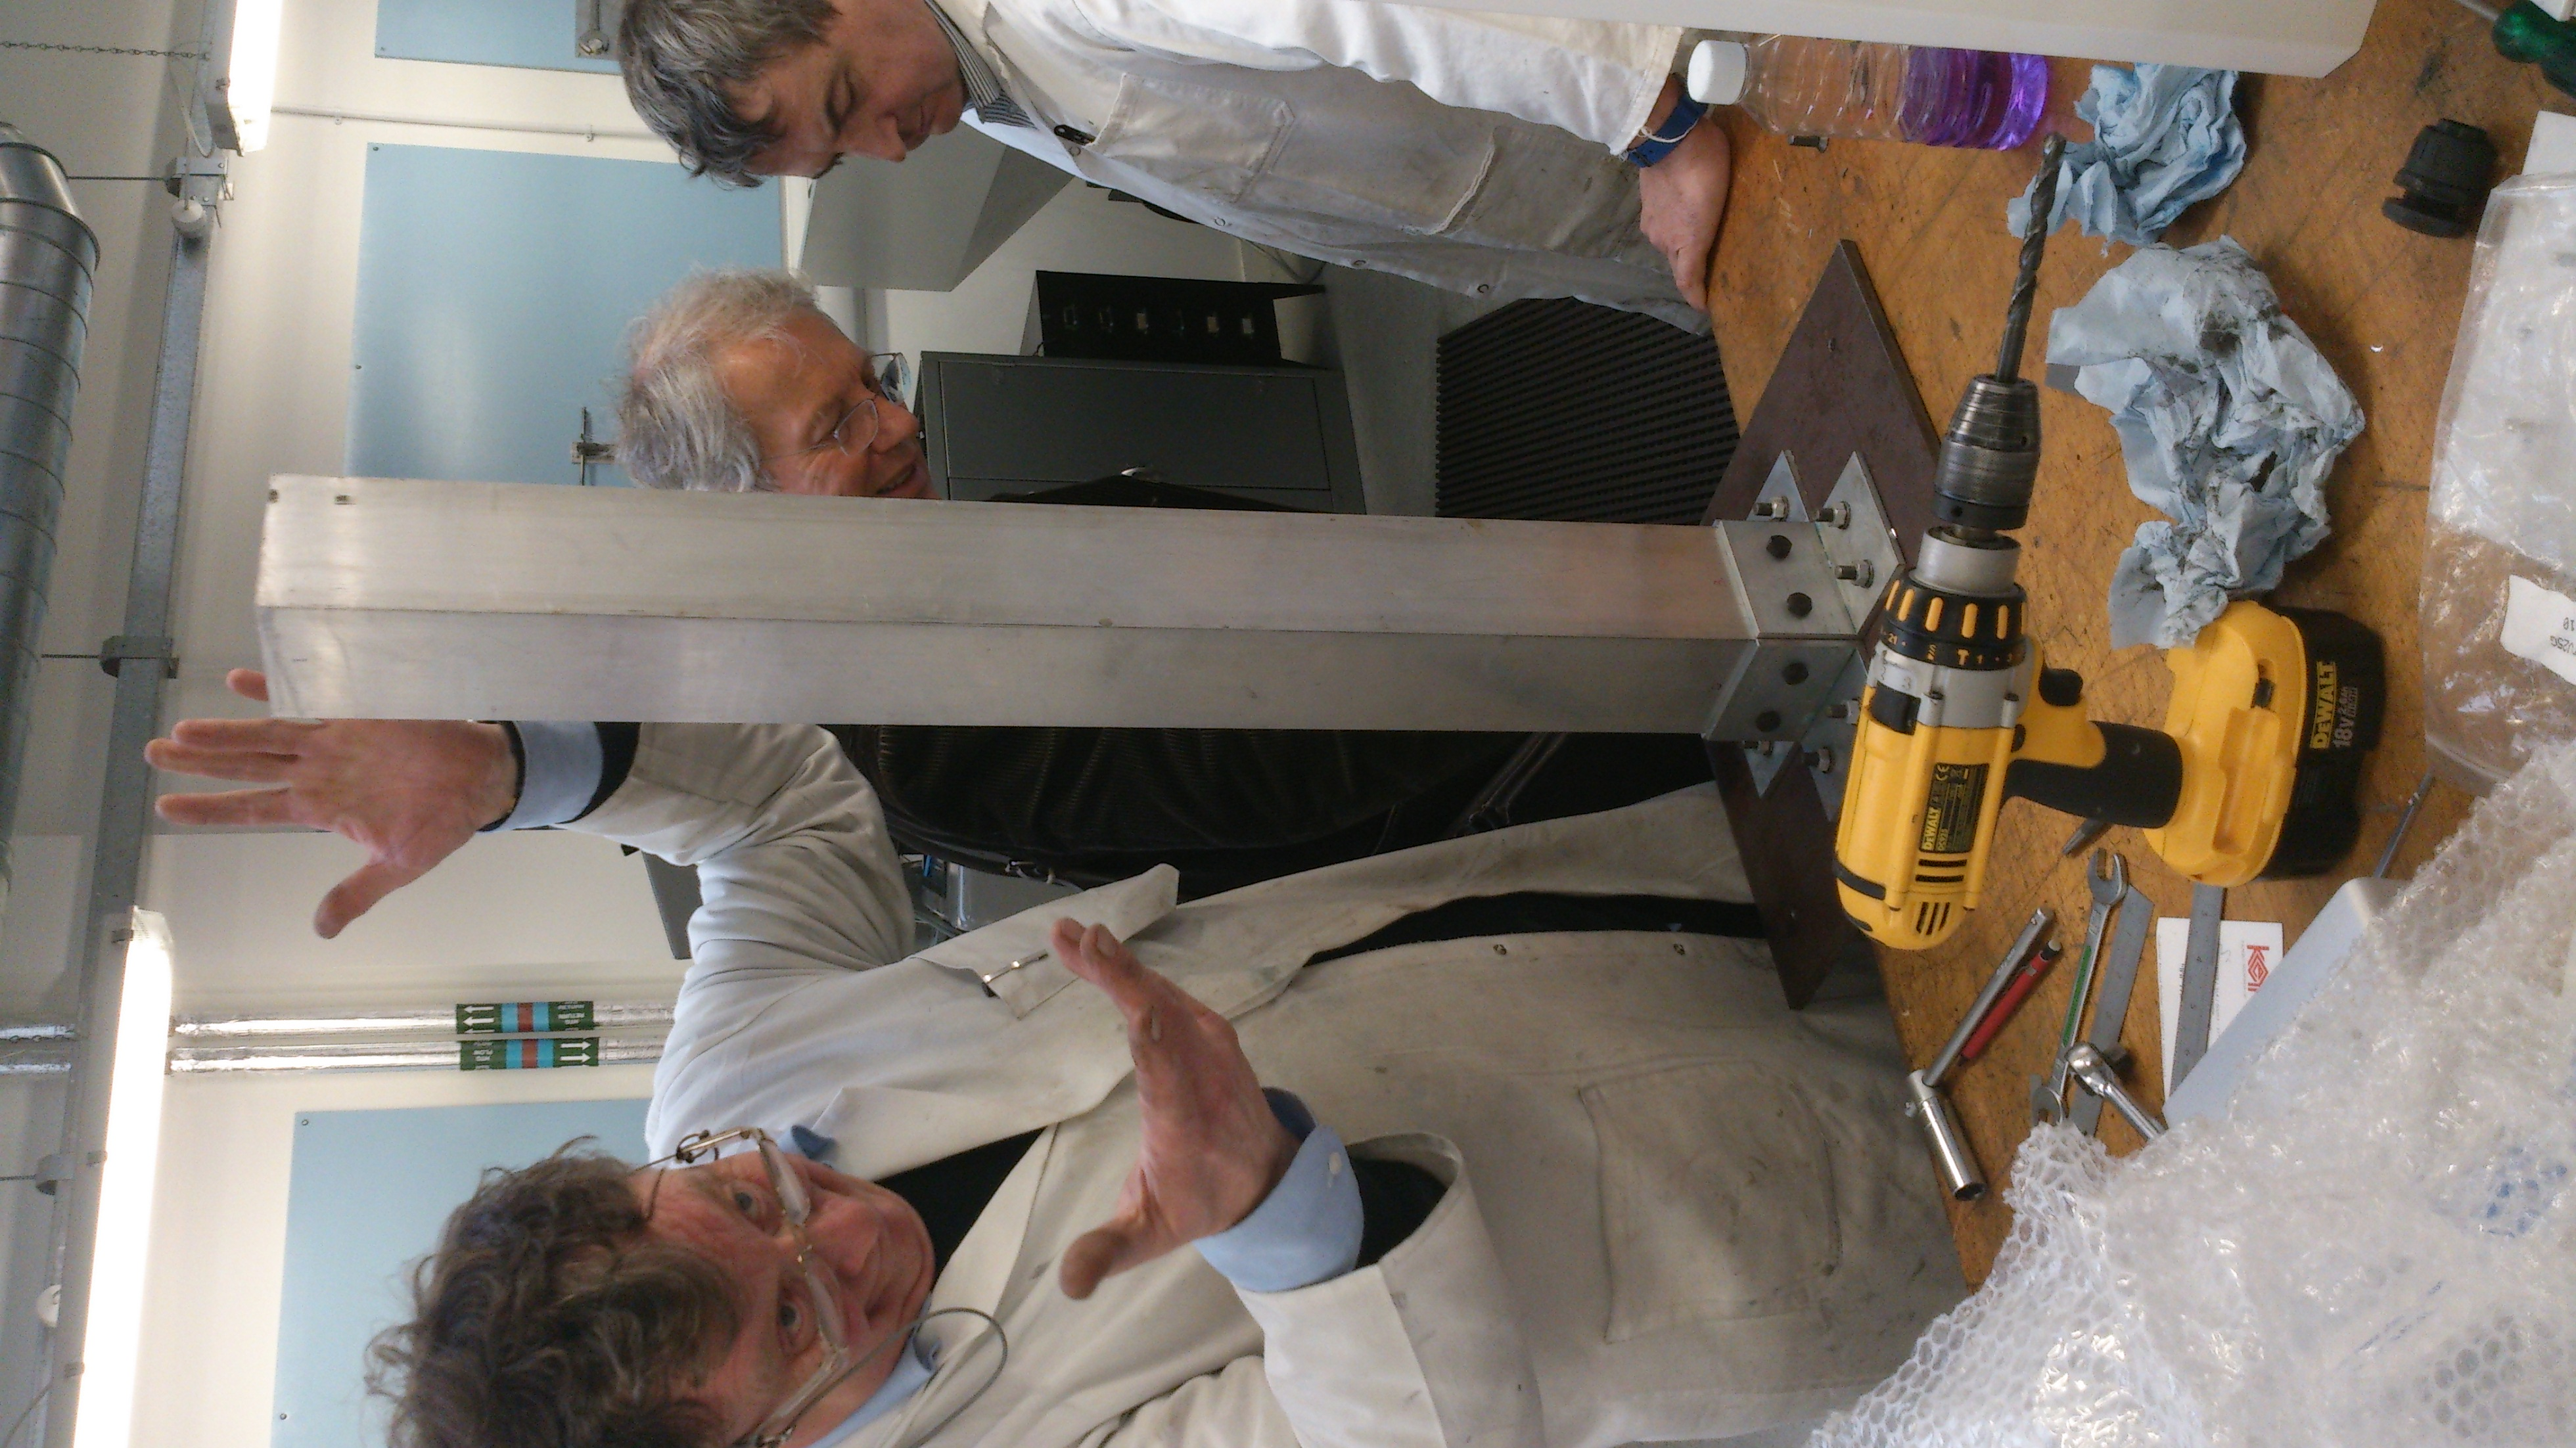
\includegraphics[angle=-90,width=0.3\textwidth]{tada}
\end{wrapfigure}
Story about trials and tribulations of getting them mounted...

And also how they had to have the glass screwed down because it came
off very easily...

\begin{figure}[h]
  \begin{center}
    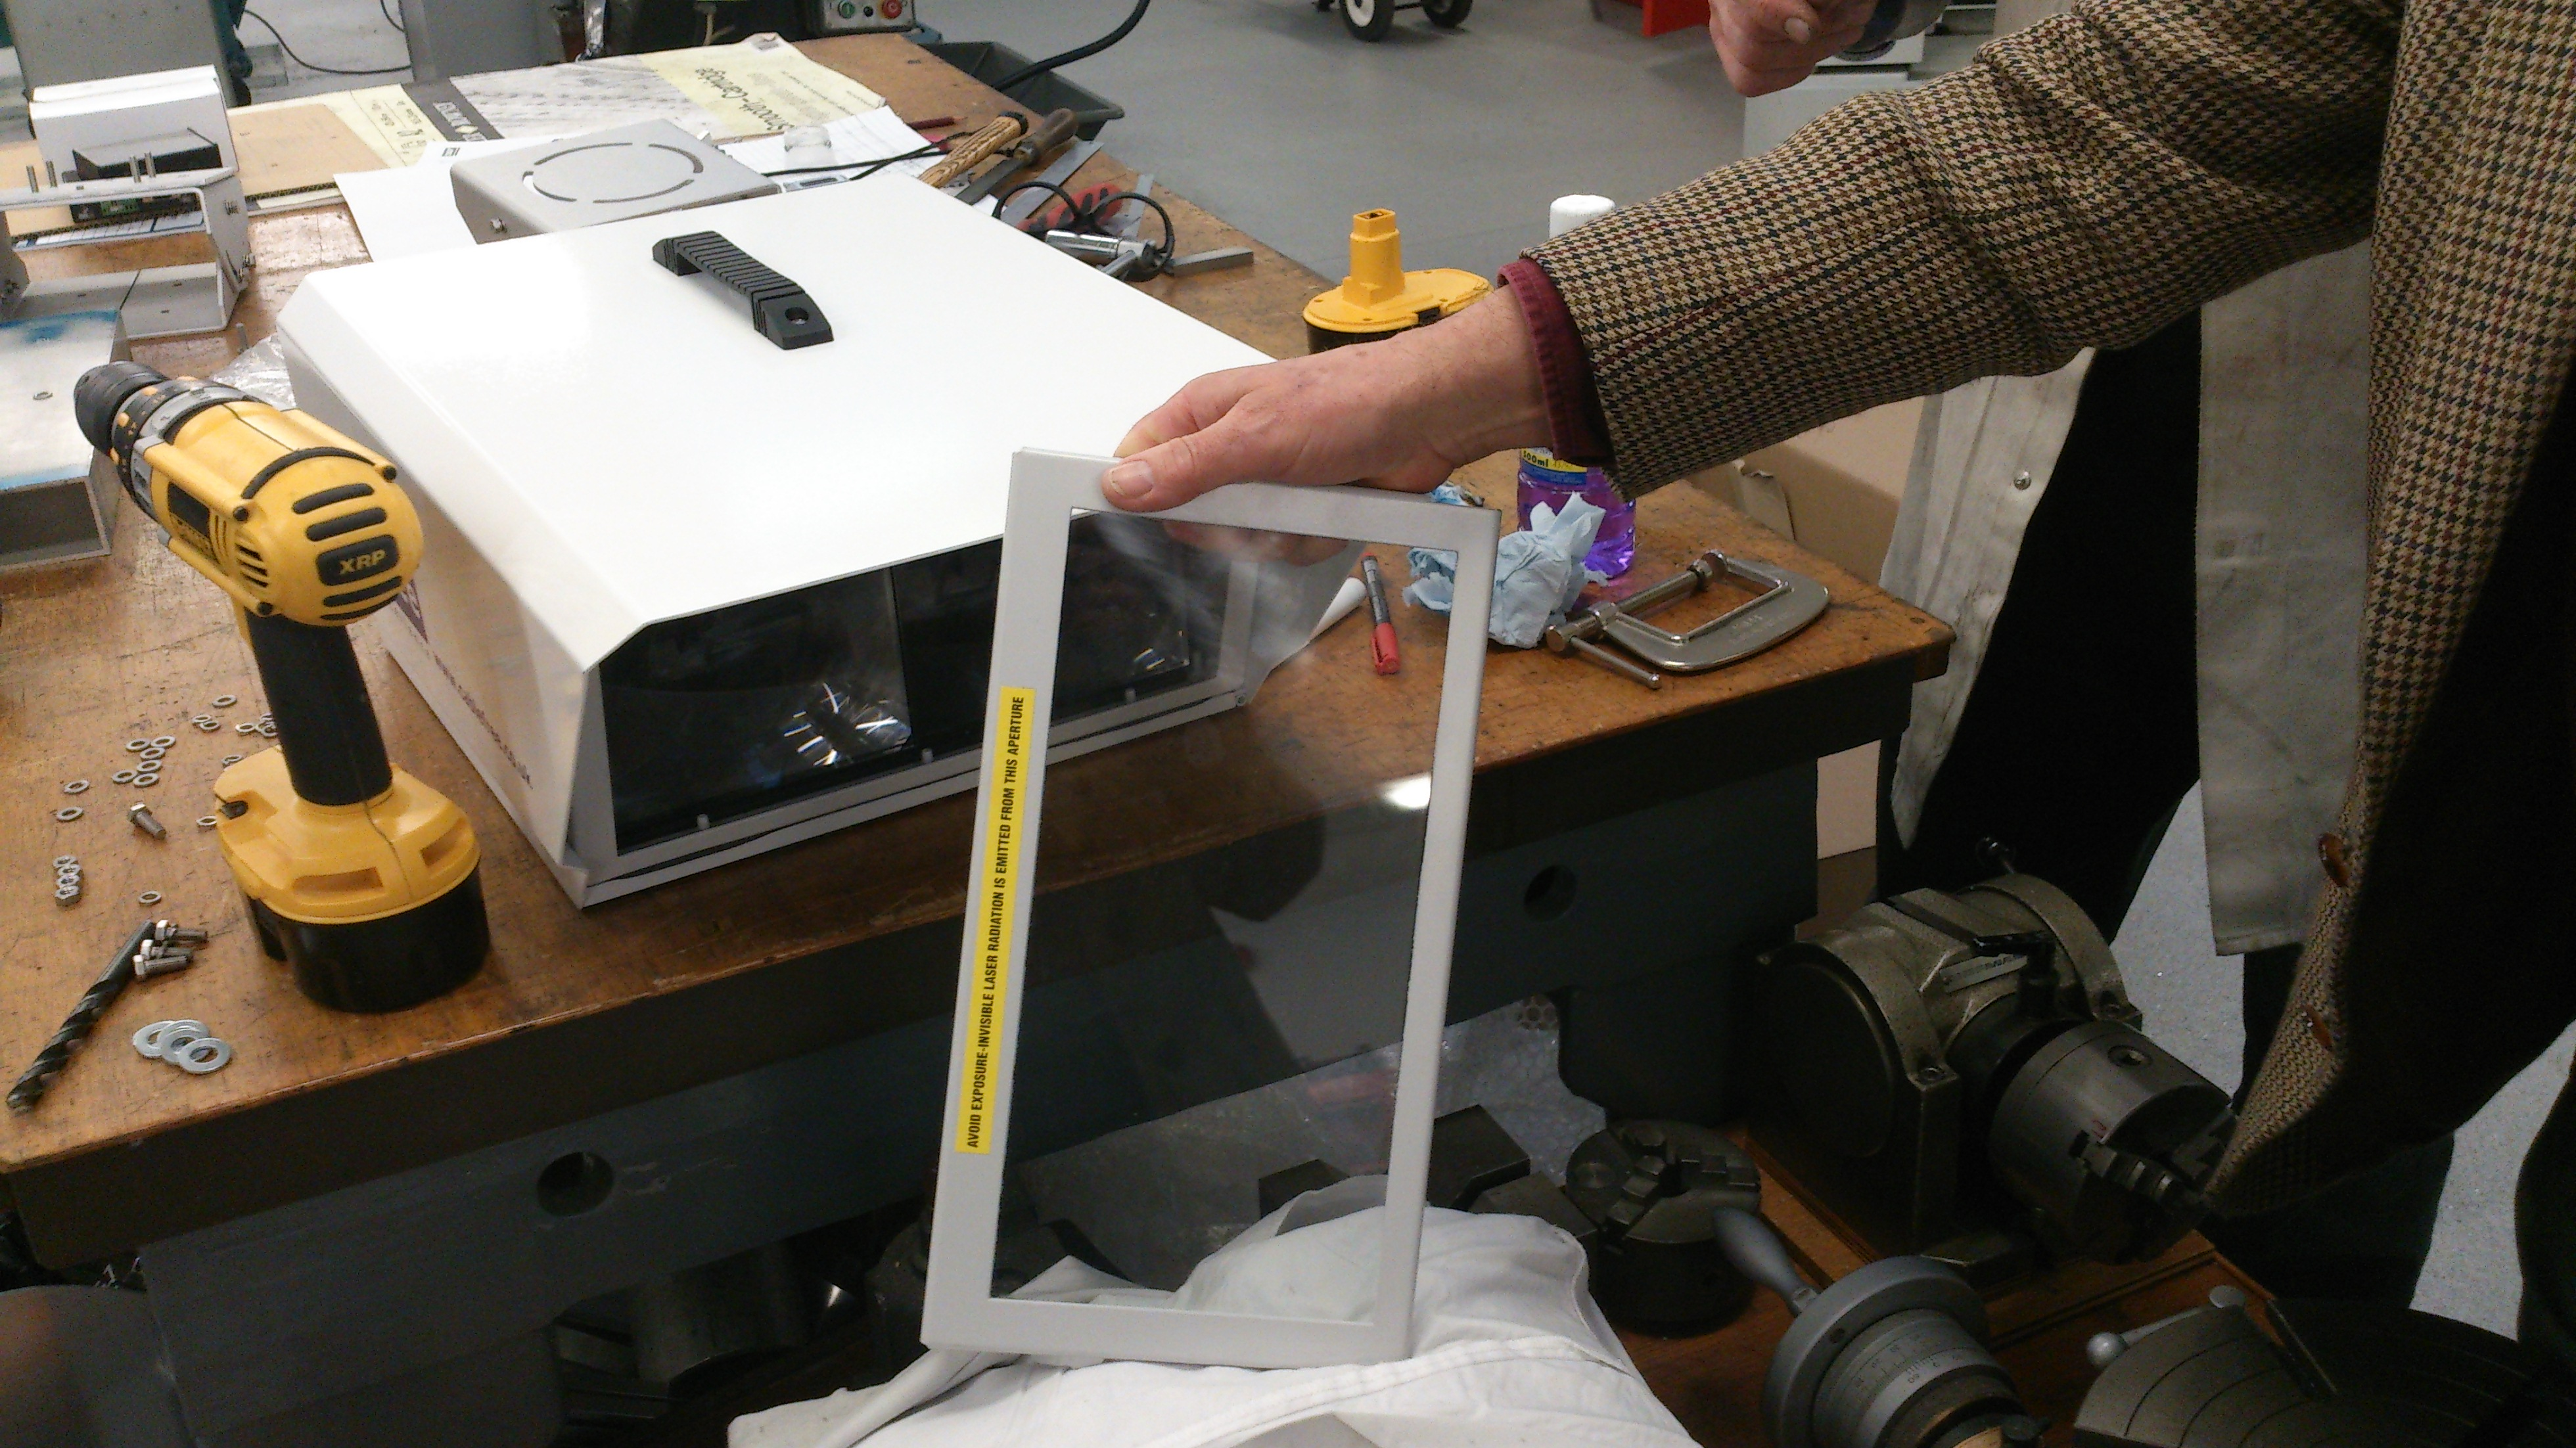
\includegraphics[width=0.5\textwidth]{faulty}
  \end{center}
\end{figure}

%%% Local Variables:
%%% mode: latex
%%% TeX-master: "scotgov-report"
%%% reftex-default-bibliography: ("literature.bib")
%%% zotero-collection: #("28" 0 2 (name "Papers/Scotgov Report"))
%%% End:

\end{document}
